%*******10********20********30********40********50********60********70********80
%% ----------------------------------------------------------------
%% Thesis.tex -- MAIN FILE (the one that you compile with LaTeX)
%% ---------------------------------------------------------------- 

%% This template is based on Graduate Thesis written by Sunil Patel,
% (ho based it on the ecsthesis template) under the LaTeX Project Public License.
% which can be found here: http://latex-project.org/lppl/
% in the hope that it will be easier to use and to scale down to your needs
% by Simon Ternsjö in 2013-10



% INSTRUCTIONS:

% The meaning is not to edit this document much, but to fill in information 
% in the different files in the folders;
% Settings, Frontpages, Chapters, Appendices and possibly Files,
% as well as the file Bibliography.bib

% This template is easy to scale down to suite your need, 
% simply comment the input statements explained below


% Set up the document:
\documentclass[a4paper, 11pt, oneside]{Thesis}  % Use the "Thesis" style, based on the ECS Thesis style by Steve Gunn

% Add more package in Package.tex:
% Add your own packages here, 
% these existing packages can be removed if necessary
% not that more packages are imported in Thesis.cls, '
%  but those should not be changed if you don't know what you are doing...


\usepackage[utf8]{inputenc} % for writing other that basic characters
\usepackage{graphicx}
\usepackage{caption}
\usepackage{subcaption}
\usepackage{multicol}
\usepackage[dvipsnames*,svgnames]{xcolor}
\usepackage{listings}
\usepackage{hyperref}
\usepackage{float}

% Include any extra LaTeX packages required
\usepackage[square, numbers, comma, sort&compress]{natbib}  % Use the "Natbib" style for the references in the Bibliography
\usepackage{verbatim}  % Needed for the "comment" environment to make LaTeX comments
%5%\usepackage{vector}  % Allows "\bvec{}" and "\buvec{}" for "blackboard" style bold vectors in maths




% Use if you want:
%5%\graphicspath{Figures/}  % Location of the graphics files (set up for graphics to be in PDF format)
%5%\hypersetup{urlcolor=blue, colorlinks=true}  % Colours hyperlinks in blue, but this can be distracting if there are many links.

% Set your name, the title of the report and more in Administraitve.tex:
% This is where author, university, title and more is defined

% Personal information:
\newcommand{\myAuthorName}  {Andrea Spreafico}% Author Name
\newcommand{\myAuthorEmail} {asp005@post.uit.no} % Author email
\newcommand{\myTitle}       {Python potential in Data Science field: Norwegian salmon farming analysis.} % Thesis title goes here
\newcommand{\mySubject}     {Computer Science} % Subject goes here
\newcommand{\myKeywords}    {Aquaculture, Fishery} % Keywords goes hear



% University information
\newcommand{\myUniversity}{University of Tromsø} %The Iniversity name goes here
\newcommand{\myUniversityWeb}{https://en.uit.no/startsida} %University Web Site URL Here (include http://
\newcommand{\myDepartment}{Department of Computer Science} % The Department goes here 
\newcommand{\myDepartmentWeb}{https://en.uit.no/om/enhet/forsiden?p_dimension_id=88138} % Department Web Site URL Here (include http://)
\newcommand{\myFaculty}{Faculty of Computer Science}
\newcommand{\myFacultyWeb}{https://uit.no/utdanning/program?p_document_id=279505}

%Degree, program or corse: ex: Master of Science, Engineering Physics
\newcommand{\myDegree}{Computer Science} % The degree, program or course-name goes here


% can be left untouched, both:
\newcommand{\myDate}{\today}
\newcommand{\myPartyalFulfillment}{A thesis submitted in partial fulfillment for the degree of Computer Science}


%% ----------------------------------------------------------------
\begin{document}

\frontmatter      % Begin Roman style (i, ii, iii, iv...) page numbering


% Here the first pages are imported, you can find them in the Frontpages folder
% Files in the subfolder Fixed does not need to be edited.
% If you don't need any of these sections, simply comment, or delete, the input-row\dfrac{•}{•}


%% All the pages before the chapters ------------------------------
\input{Frontpages/Fixed/Title}

\input{Frontpages/DeclarationPage.tex}

% The "Funny Quote Page"
\clearpage
\pagestyle{empty}  % No headers or footers for the following pages

%use 1 or vfill to position the quote where it looks good:
\null\vfill\vfill


% Now comes the "Funny Quote", written in italics:

\textit{
    % Write a funny quote here:
    ''We did it, we bashed them, wee Potter’s the one, \\
    and Voldy’s gone moldy, so now let’s have fun!''
}
\begin{flushright}
    % If the quote is taken from someone, their name goes here:
    - Peeves
\end{flushright}


 
\vfill\vfill\vfill\vfill\vfill\null


% The Abstract Page
\clearpage 
\addtotoc{Abstract}  % Add the "Abstract" page entry to the Contents
\abstract{
    \addtocontents{toc}{\vspace{1em}}  % Add a gap in the Contents, 
                                        %for aesthetics
    
    %The Thesis Abstract is written here (and usually kept to just this page). 
    %The page is kept centered vertically so can expand into the blank space above the title too \ldots
    
    Moonstone (also known as the wishing stone[1]) is found in a variety of colors. Its supposed magical effects include helping a person gain emotional balance. Since Harry spent much of book five emotionally unbalanced, it is perhaps fitting that he was forced to write an essay on the stone's use in Potions-making. It is a gemstone of medium value. Moonstones are a milky colour and shine very brightly, almost as though they are a source of their own light. They are a useful potion ingredient; powdered moonstones are used as an ingredient for the Draught of Peace and in several Love Potions. Powdered Moonstone is also an ingredient in in Potion No. 86 which is likely an experimental potion. Moonstones were also known to be among the gems set into Muriel's tiara.
    

    
}



% The Acknowledgements page, for thanking everyone
\clearpage 

\chapter{Acknowledgements}
    % The acknowledgements and the people to thank go here, don't forget to include your project advisor...
    
    % The following are examples of how to word your thanks
    
    Ståle Walderhaug	\\
	Bård Johan Hanssen\\
    Sara Björk \\
	SINTEF Nord\\
 	UiT - Universitetet i Tromsø\\
 	
    I would like to express my very great appreciation to\\
    I would also like to offer my special thanks to \\
    My special thanks are extended to the staff of \\
    My special thanks goes to Pomona Sprout for taking on this thesis work.\\
    I am particularly grateful for the support and good times given by my friends \\    
    To my family, for \\
    I am particularly grateful.    \\
    Advice given by Helga Hufflepuff has been a great help in \\


 
 
 


\input{Frontpages/Fixed/TableOfContents.tex}

\input{Frontpages/Fixed/ListOfFigures.tex}

\input{Frontpages/Fixed/ListOfTables.tex}

\clearpage
\pagestyle{fancy} % The page style headers have been "empty" all this time, 
                  % now use the "fancy" headers as defined before
\setstretch{1.5} % Set the line spacing to 1.5, 
                 % this makes the following tables easier to read
\lhead{\emph{Abbreviations}}  % Set the left side page header to "Abbreviations"
\listofsymbols{ll}  % Include a list of Abbreviations (a table of two columns)
{
  % \textbf{Acronym} & \textbf{W}hat (it) \textbf{S}tands \textbf{F}or \\
   \textbf{LAH} & \textbf{L}ist \textbf{A}bbreviations \textbf{H}ere \\
   \textbf{OWL} & \textbf{O}rdinary \textbf{W}izarding \textbf{L}evel\\
}


% \input{Frontpages/PhysicalConstants.tex}

% \input{Frontpages/Symbols.tex}

\clearpage
\lhead{}  % Set Left page header to nothing.
\setstretch{1.3}  % Return the line spacing back to 1.3
\pagestyle{empty}  % Page style needs to be empty for this page


\dedicatory{For/Dedicated to/To my\ldots}


\addtocontents{toc}{\vspace{2em}}  % Add a gap in the Contents, for aesthetics




%% The Body -------------------------------------------------------
\setstretch{1.3}  % Return the line spacing back to 1.3
\mainmatter	  % Begin normal, numeric (1,2,3...) page numbering
\pagestyle{fancy}  % Return the page headers back to the "fancy" style


% Include the chapters of the thesis, as separate files
% Just uncomment the lines as you write the chapters


%*******10********20********30********40********50********60********70********80

\chap{Introduction}

During the last few years we have witnessed an ever-increasing production of data in any sector all around the world.
For this reason instruments and techniques for analyzing and understanding these data are becoming more and more indispensable, in order to extract useful information that might be used to improve business strategies or people's life condition.

Data Science is a recent launch field which contains processes and systems that could be used to extract knowledge from data, either structured or unstructured. Since the newness of this field, would be very interesting to test and evaluate different ways to apply daily technologies to its procedures and systems.

Python is a simple interpreted, object-oriente and high-level programming language that has a easy to learn syntax.
Since it provides severals modules and package, the use of Python during a Data Science process could be very productive.

The processes and systems which belong to the Data Science field might be applied to high-interest  economic areas, such as the Aquaculture industry in Norway.
This business, in particular the Norwegian salmon farming, has a big economic repercussions on the country, and at the same time is producing a huge amount of data, so it would be very helpful to restructure and analyze it.

This thesis will contributes providing a documented implementation of an analysis, displaying and prediction system using Python applied to the Norwegian salmon farming.

\newpage

\section{Aim of the study}
\vspace{-5mm}
The focus of this study will be on:
\begin{itemize} 
 \item Initial approach with Data Science field, in order to investigate and document possible techniques, methods and approaches.
 
 \item Testing Python potential in Data Science field, describing implementation procedures and reporting pro and cons. 
 
 \item Report the initial analysis and displaying results about Norwegian salmon farming, in order to provide structured, described and readable data that might be used for future works.
\end{itemize}

\section{Research Objectives}
\vspace{-5mm}
The above aim will be accomplished by fulfilling the following research objectives:

\textbf{1) Collect as much data about aquaculture in Norway as possible.}
\vspace{-5mm}
\begin{itemize}
 \setlength{\itemsep}{-5pt}
  \item Which kind of data is possible to obtain about aquaculture general statistics in Norway? Where is possible to find it? Are that available for everyone?
  \item Which kind of data is possible to obtain about aquaculture of single locations in Norway? Where is possible to find it? Are that available for everyone?
\end{itemize}

 
\textbf{2) Increase accessibility and availability of the data.}
\vspace{-5mm}
\begin{itemize}
 \setlength{\itemsep}{-5pt}
  \item How you can create a unique dataset that contains and summarize all the data previous collected?
  \item Which kind of structure allows to the total dataset to be more accessable and readadble than the original single sources?
\end{itemize}
 
\textbf{3) Analyze and display the data.}
\vspace{-5mm}
\begin{itemize}
 \setlength{\itemsep}{-5pt}
  \item Which kind of Python functions is possible to use for analyze and displaying data? 
  \item Which kind of requirements does it need and how is possible to implement it?
  \item Why Python could be a good solution for data analysis and displaying? 
  \item Which kind of relationships and patterns about the data is possible to identify using the result graphics? How is possible to identify it?
  \item How is possible to check out the data trend line? 
  \item Which kind of informations have been reported for future reuse? How it's possible to access it? (Informations such as correlation coefficients, trend line equations,..)
 \end{itemize}

\newpage

\textbf{4) Extract information from the data.}
\vspace{-5mm}
\begin{itemize}
 \setlength{\itemsep}{-5pt}
  \item Which parameters about aquaculture in Norway are increasing? How fast are they increasing/decreasing? 
  \item How you can compare different parameters trend line?
  \item Which kind of correlations is possible to find out between different parameters? How is possible to show it? What is possible to extract from that?
 \end{itemize}
 
\textbf{5) Prediction of values about the data.}
\vspace{-5mm}
\begin{itemize}
 \setlength{\itemsep}{-5pt} 
  \item Which kind of Python utilities is possible to use for time series predictions?
  		\vspace{-3mm}
		\begin{itemize}
 		\setlength{\itemsep}{-5pt}	
		  \item How Python works for time series prediction systems implementation?
		  \item Which kind of accuracy it provides about the predicted values?
		  \item Would it be a good way for let the people get some experience with the machine learning field? 
		\end{itemize}
  \item Would be useful to have the possibility of forecasting some future data? 
  \item Which kind of data might be the most useful to know for people into the Aquaculture field?
	
 \end{itemize}

\textbf{6) Recommendations to future work and extra ideas.}
\vspace{-5mm}
\begin{itemize}
\setlength{\itemsep}{-5pt}
	\item How it could be possible to improve the Anaysis and Displaying system?
	\item How it could be possible to improve the Forecasting system?
	\item Which kind of services is possible to provide using the collected informations and the implemented systems?
  		\vspace{-3mm}
		\begin{itemize}
 		\setlength{\itemsep}{-5pt}	
		  	\item How you can provide the analysis system like a service?
		  	\item How you can provide the prediction system like a service?
		\end{itemize}
 \end{itemize}

\newpage

\section{Thesis Structure}
\label{Thesis_Strucutre}
\textbf{Background Theory}\\
Here is report the relevant background theory that should be needed for better understand the work done during this thesis.

\textbf{I Part: Data collection and validation}\\
During this initial part of the work the main purpose is to collect as much data as possible. The data have to be related with the current are of interested and at the same time considered reliable. Once collected enough data, is time to describe and structure them in a proper dataset.


\textbf{II Part: System implementation}\\
During this part of the work is implemented the Python system and reported the procedure, in order to try to find as many answers as possible to the initial goals. The implemented system will be divided in several subsystems, that's because it allows an easier implementation procedure and a higher reusability. It's possible to checkout an overview about the implemented subsystems in the next section. [\ref{System_Design}]


\textbf{III Part: Result, Discussion and Conclusions }\\
In the current part of the study are reported the results and the relative interpretations. Further more, is reported a general sumamrize about the study and also any kind of evaluations, challenges, limitations encountered and some recommendations for future works.


\textbf{IV Part: Full code Implementation }	\\
In this last part of the study is reported the full commented code implementation for each single system implemented. It would be useful to checkout more details about the code, since during the II Part is reported just the most important rows and functions of the code.


\section{Previous Works}
\vspace{-5mm}
The implementation of the prediction system in this thesis was based on a previous work, which provides a basic implementation of a forecasting system with Python.\\
That particular work was showing how to create a general ARIMA Model for Time Series Forecasting with Python. During this study that implementation has been improved, customized and applied to the current context.

The previous work source website is named "machinelearningmastery.com", and here's the reference: \cite{previousWork}


\section{Work repository}
\label{Repository}
Before start to read the implementation procedure about this work, it's important to know that is possible to check out the system's full implementation on Github.\\
I suggest to check it out and download the following repository. It allows to test the system and better understand how it is structured and how it works.\\
Further more, it's possible to find inside the same repository all the needed datasets and a "Manual" wich contains the instructions about how to use it.

The Github repository is:\\
\url{https://github.com/Sprea22/Python_Systems}

The direct Zip file download is:\\
\url{https://codeload.github.com/Sprea22/Python_Systems/zip/master}

 % Introduction
%*******10********20********30********40********50********60********70********80

\chap{Background Theory} 
\section{Data science}
\vspace{-5mm}
It's really important to have a general idea about what "Data Science" means since this thesis procedure is strongly based on the classic Data Science Process.

We can define Data Science like a "concept to unify statistics, data analysis and their related methods" in order to understand and analyze actual phenomena with data.\cite{wiki:DataScience}\\
It includes theories drawn from many field within the broad areas of mathematics, statistics, information science and computer science.
In the computer science area are particular important the subdomains of:\\

\begin{minipage}{0.5\textwidth}
\textbf{Machine learning}: Is a subfield of computer science that gives computers the ability to learn without being explicitly programmed \cite{ArthurSamuel}. More useful specific informations about this field are provided in the following section [\ref{ML}].\\

\textbf{Cluster Analysis}: is the task of grouping a set of objects in such a way that objects in the same group (called a cluster) are more similar (in some sense or another) to each other than to those in other groups (clusters) \cite{wiki:clusterAnalysis}. \\ 


\end{minipage} \hfill
\begin{minipage}{0.50\textwidth}
\begin{figure}[H]
	\centering
    \includegraphics[trim={0 3cm 0 4cm},clip,width=0.8\textwidth]{Files/Data_Science_Concept.pdf}
    \caption{Data science concept}
    \label{fig: Data_science}
\end{figure}
\end{minipage}


\textbf{Classification}: Is the problem of identifying to which of a set of categories (sub-populations) a new observation belongs \cite{wiki:Classification}. 


\textbf{Data mining}: Is the computing process of discovering patterns in large data sets. The overall goal of the data mining process is to extract information from a data set and transform it into an understandable structure for further use. 

\textbf{Databases}: A database is an organized collection of data. It is the collection of schemas, tables, queries, reports, views, and other objects. The data are typically organized to model aspects of reality in a way that supports processes requiring information. \cite{wiki:Databases}

\textbf{Data Visualization}: It involves the creation and study of the visual representation of data. The primary goal of data visualization is to communication information clearly and efficiently via graphics and plots. \\



This study procedure is strongly based on the Data Science process designed by Joe Blitzstein and Hanspeter Pfister \cite{DataProcessFramework}, which is reported in the following image.
\begin{figure}[H]
    \centering
    \makebox[\textwidth][c]{\includegraphics[trim={0 0 0 2cm},clip, width=1.2\textwidth]{Files/Data_Science_Process.pdf}}
    \caption[Data science process]{Data science process}
    \label{fig: Data_science_process}
\end{figure}

\newpage


\section{Machine learning}
\vspace{-5mm}
\label{ML}
As reported in the previous section, this subfield of computer science gives "computers the ability to learn without being explicitly programmed". \\
Machine learning explores the study and construction of algorithms that can learn from and make predictions on data.

There are several machine learning algorithms, each one of them is used for a different purpose and a different domain. For examples:
  \vspace{-5mm}
\begin{itemize}
 
  \item Artificial Neural Network: Computations are structured in terms of an interconnected group of artificial neurons. They are usually used to model complex relationships between inputs and outputs, to find patterns in data or to capture statistical structures. 
  
  \item Deep Learning: This concept consists of multiple hidden layers in an artificial neural network, and it can be successfully applied for computer vision and speech recognition.
  
  \item Clustering: Is the assignment of a set of observations into subsets, called clusters, so that observations within the same cluster are similar according to some predesignated criteria, while observations drawn from different clusters are dissimilar.
  
  \item \textbf{Regression}: Is a statistical process for estimating the relationships among variables. It includes many techniques for modeling and analyzing several variables, when the focus is on the relationship between a dependent variable and one or more independent variables. Regression analysis is widely used for prediction and forecasting, where its use has substantial overlap with the field of machine learning. This specific domain contains the model used in this study \cite{wiki:Regression}.
  
  \item Bayesian:
  
 \end{itemize}  

\newpage

\subsection{Time Series analysis and predictions}
  \vspace{-5mm}
Time Series forecasting is an important area of machine learning, but that is often neglected. Is that important mainly beause there are so many prediction problems that involve a time component, and these problems are neglected because it is this time component that makes time series problems more difficult to handle \cite{previousWork}.

" A time series is a sequence of observations taken sequentially in time \cite{TimeSeries}. " 

Classic example of a time series dataset:

\begin{tabular}{ | l | l | }
\hline 		\textbf{Date}	&	\textbf{Paramater} \\ \hline
				Time \#1	&	observation \\ \hline	
				Time \#2	&	observation \\ \hline	
				Time \#3	&	observation \\ \hline											
\end{tabular}

Understanding a dataset is called time series analysis and it can helps to make better prediction, but sometimes it's not required and can result in a large of technical investment in time and expertise.

Making predictions could be called time series forecasting and it involves taking models fit on historical data and using them to predict future observations.

\subsection{Autoregressive integrated moving average (ARIMA)}
\vspace{-5mm}
A widely used statistical method for time series forecasting is the ARIMA model. Since this a very complicated and deep topic, this study provided just an initial implementation and description of it. During this section are provided some basic definitions and overviews enough to understand the general logic behind a forecasting system. If you are particularly interested in this topic my suggestion is to read more about it, in the specific the mathematic side.

\textbf{AR model}: an autoregressive model is a representation of a type of random process; as such, it is used to describe certain time-varying processes in nature, economics, etc. The autoregressive model specifies that the output variable depends linearly on its own previous values and on a stochastic term (an imperfectly predictable term); thus the model is in the form of a stochastic difference equation.\cite{wiki:AR}

\textbf{MA model}: a moving-average model is a common approach for modeling univariate time series. The moving-average model specifies that the output variable depends linearly on the current and various past values of a stochastic (imperfectly predictable) term.\cite{wiki:MA}

\newpage

\textbf{ARMA model}: an autoregressive-moving-average model provides a parsimonious description of a stationary stochastic process in terms of two polynomials, one for the autoregression and the second for the moving average. Basically it combines both AR and MA models into a unique representation.\cite{wiki:ARMA}

\textbf{ARIMA model}: is a generalization of an autoregressive moving average (ARMA) model. Both of these models are fitted to time series data either to better understand the data or to predict future points in the series (forecasting).\\
This model is applied in some cases where data show evidence of non-stationarity, where an initial differencing step (corresponding to the "integrated" part of the model) can be applied one or more times to eliminate the non-stationarity.\cite{wiki:ARIMA}

\textbf{ARIMA(p, d, q)}
  \vspace{-5mm}
\begin{itemize}
 \setlength{\itemsep}{-5pt}
\item \textbf{p} is the number of autoregressive terms (How many preceding values are examinated for the current value’s forecast).

\item \textbf{d} is the number of nonseasonal differences needed for stationarity.

\item \textbf{q} is the number of lagged forecast errors in the prediction equation. 
\end{itemize}

\newpage

\section{Aquaculture in Norway}
\vspace{-5mm}
During the last years there has been a very rapid development of Norway's aquaculture industry, and the production of Atlantic salmon has grown to become a major sector of its economy. The industry is now an economic pillar for several Norwegian coastal communities.\cite{SenCanada}

The Aquaculture industry in Norway is dominated by its finfish sector, with Atlantic salmon and Rainbow trout accounting for 93.9\% and 5.8\% respectively of total volume produced.

This business takes place in the counties along most of the country's coastline. In the fish sector Nordland is the dominant producer county, with Hordaland coming second, Møre og Romsdal third, and Troms fourth.

\begin{figure}[h]
    \makebox[\textwidth][c]{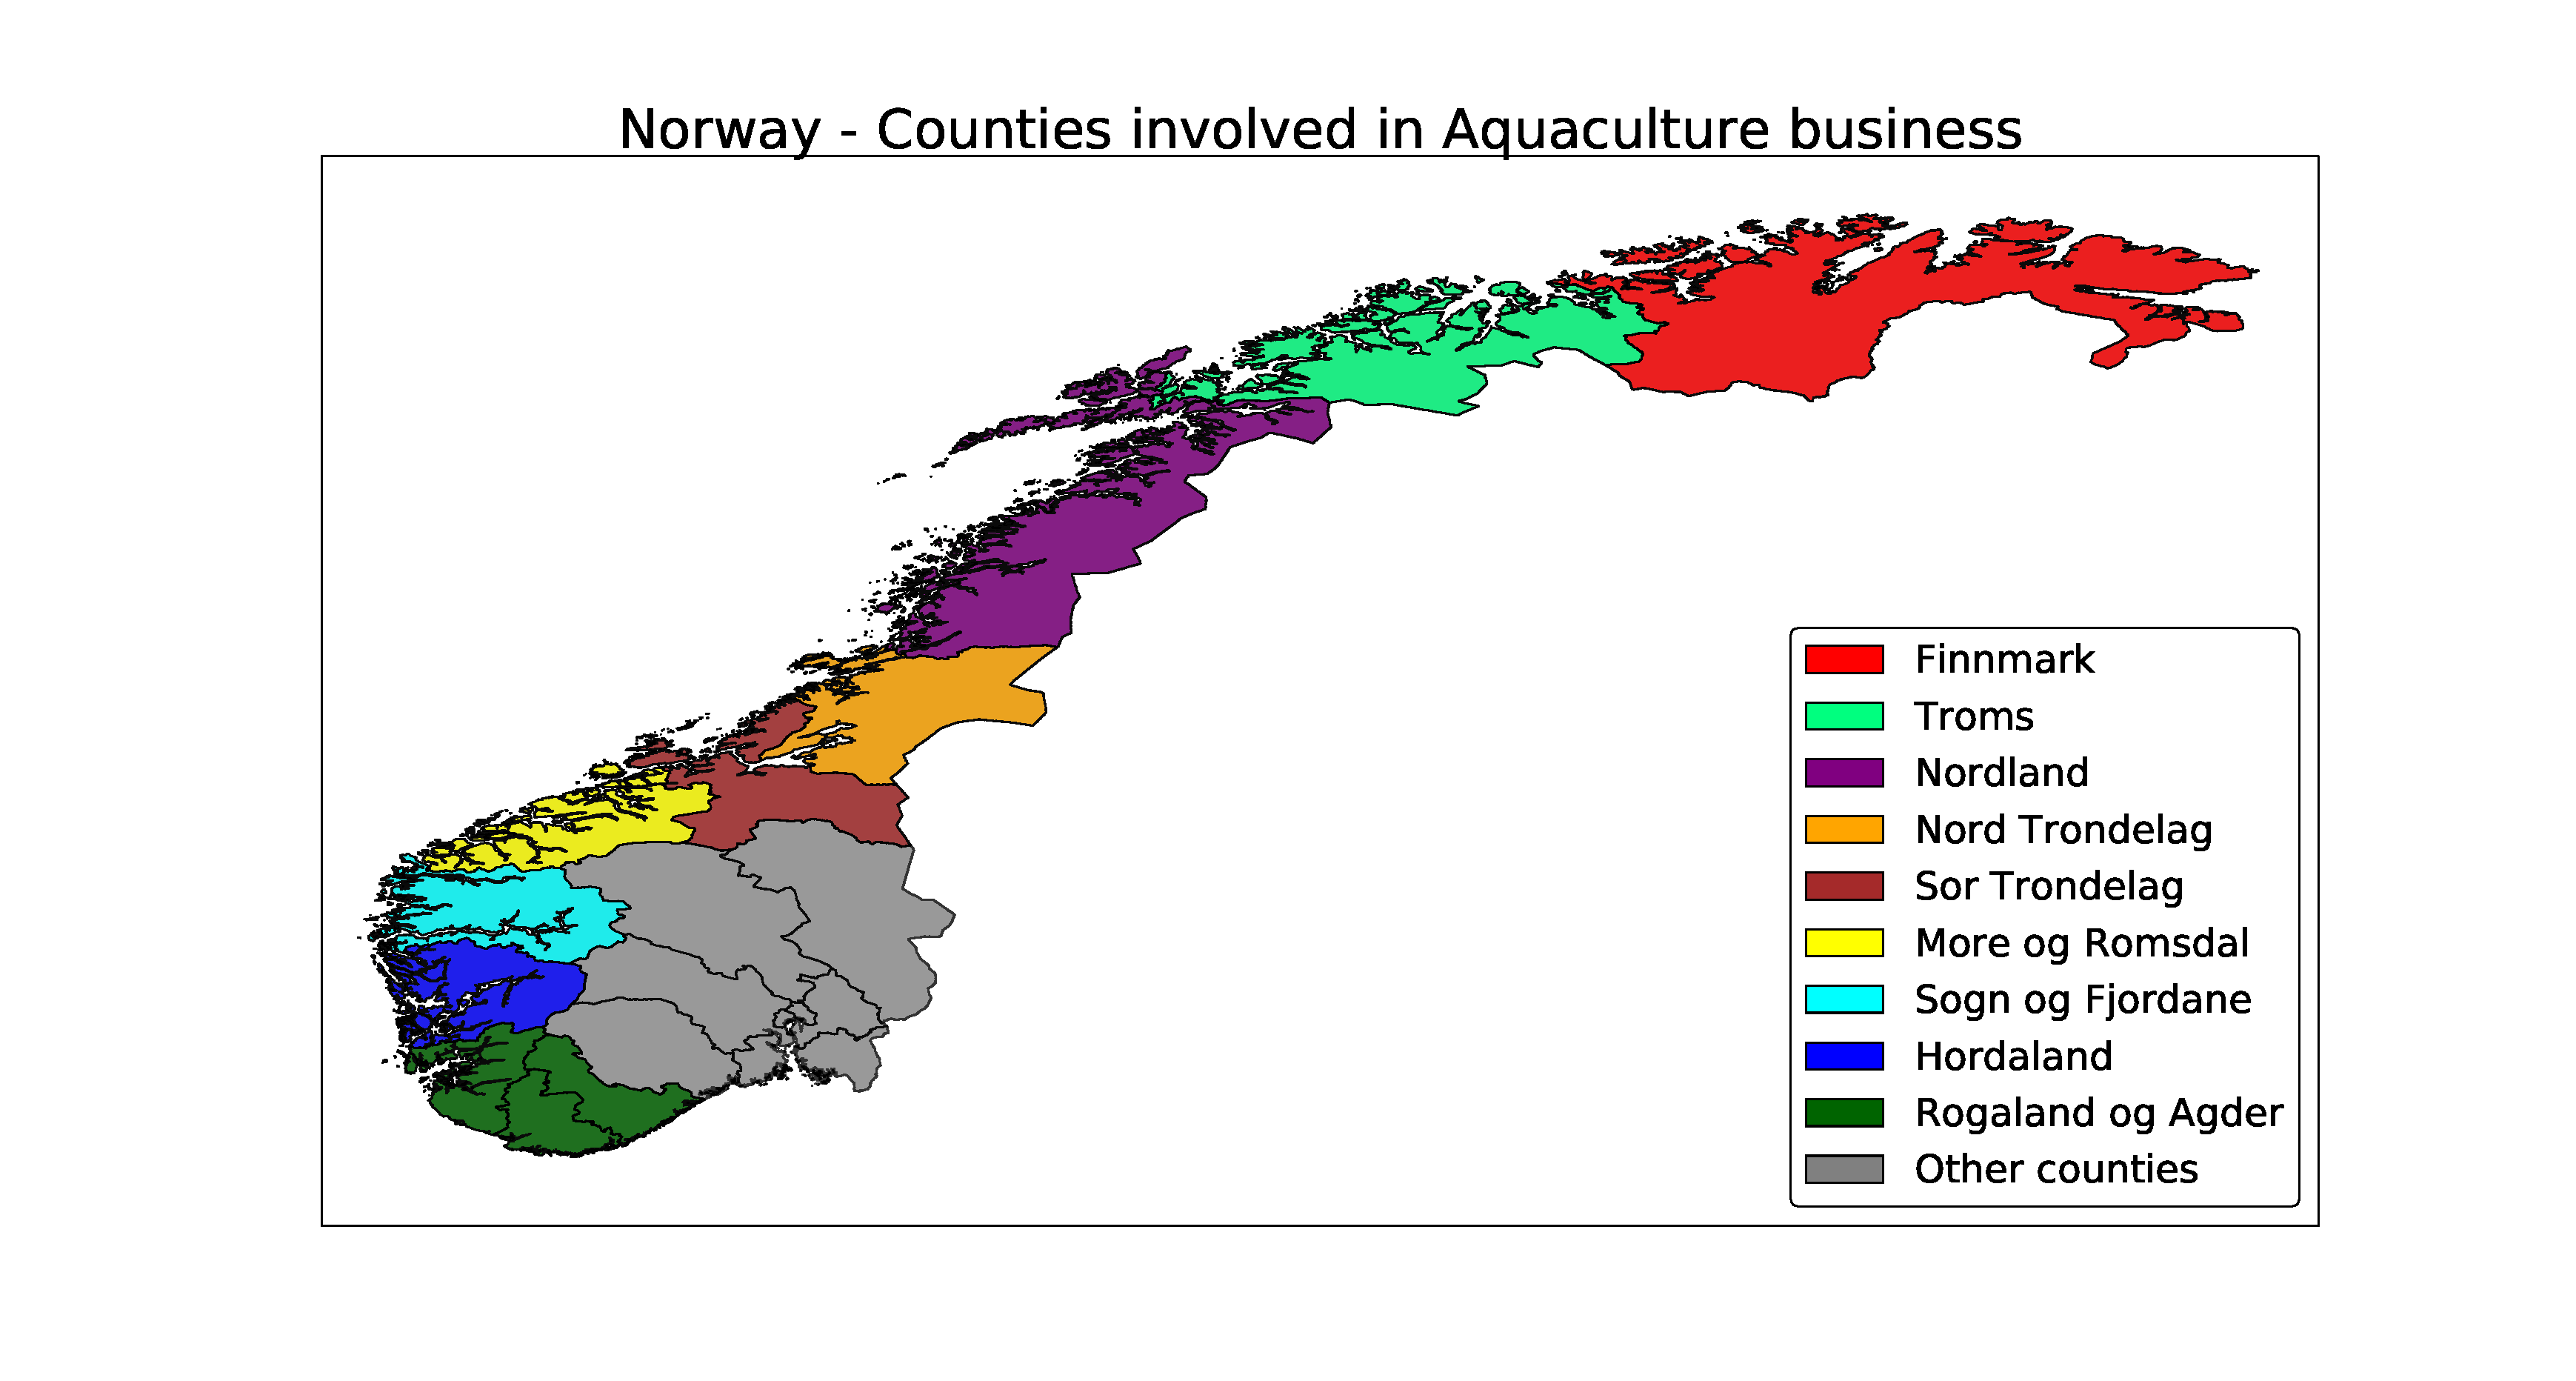
\includegraphics[width=1.2\textwidth, trim={0 0 0 0cm},clip,]{Files/Counties.pdf}}
    \caption[Norwegian counties involved in aquaculture business]{Norwegian counties involved in aquaculture business}
    \label{fig: Norway_Counties}
\end{figure} % Background Theory 
%*******10********20********30********40********50********60********70********80
\DeclareFixedFont{\ttb}{T1}{txtt}{bx}{n}{12} % for bold
\DeclareFixedFont{\ttm}{T1}{txtt}{m}{n}{12}  % for normal
\definecolor{deepblue}{rgb}{0,0,0.5}
\definecolor{deepred}{rgb}{0.6,0,0}
\definecolor{deepgreen}{rgb}{0,0.5,0}

% Python style for highlighting
\lstset{
	backgroundcolor = \color{Ivory},
    language=Python,
    basicstyle=\footnotesize,
    otherkeywords={self},             
    keywordstyle=\footnotesize\color{deepblue},
    emph={__init__},          
    emphstyle=\footnotesize\color{deepred},    
    stringstyle=\color{deepgreen},
    frame=single,                         
    showstringspaces=false  ,
    breaklines=true,
    numbers=left,
    numberstyle=\footnotesize,
    tabsize=3,
    breakatwhitespace=false
}



% For all chapters, use the newdefined chap{} instead of chapter{}
% This will make the text at the top-left of the page be the same as the chapter

\chap{Approach and Design}
\section{Development Flow}
\vspace{-5mm}
\textbf{I Part: Data collection and validation}
\vspace{-5mm}
\begin{itemize}
 \setlength{\itemsep}{-5pt}
 \item Collect as many useful data as possible.
 \item Create a structured dataset that contains the collected data.
 \item Let the new data structure be accessable, available and readable.
 \item Let the data structure be an appropriate input to the analysis system used during the study.
\end{itemize}


\textbf{II Part: Systems implementation}
\vspace{-5mm}
\begin{itemize}
 \setlength{\itemsep}{-5pt}
 \item Analysis and displaying system implementation and results collection..
 \item Informations extraction.
 \item Prediction system implementation and results collection.
\end{itemize}


\textbf{III Part: Result, Discussion and Conclusions }
\vspace{-5mm}
\begin{itemize}
 \setlength{\itemsep}{-5pt}
 \item Results:
 \item Discussion:
 \item Conclusions:
\end{itemize}


\textbf{IV Part: Full code Implementation }

\newpage

------> I PART
During this phase the most important thing is to gather as much data as possible. The data have to be of course related with the current area of interest and they should be considered somehow useful for asnwering the initial questions of the study.\\
At the same time they should be as much reliable as possible since they are indispensable for the next phases and in particular for the final results and conclusions.\\
The data’s reliability mainly depends by which source they are coming from.\\
Then you should elaborate the data that you collected in order to:

------> II PART
This phase of the work will investigate about different ways for understanding and extracting information from the data.
For instance, the data will be displayed on different kind of graphics in order to increase their readable. Further more, several coefficients will be calculated and reported, always to allow the informations extraction from the data.
During this phase the main purpose is to predict some kind of useful data about the current dataset. To reach this goal, is first of all indispensable to choose a prediction system to implement. \\
Once the prediction system has been implemented, it's time to apply it on the current data and try to get as much evidences as possible.

------> III PART
The results part contains

The purpose of the discussion is to interpret and describe the significance of this thesis results. Further more, has to be reported a critical evaluation about the work done and explain any kind of limitations found during the procedure.
The conclusion part has to contains a summarize about what was done in this thesis, and then figure out some other extra ideas, implementations or recommendations to future work about this thesis.\\
\begin{figure}[h]
    \makebox[\textwidth][c]{\includegraphics[width=1.1\textwidth,natwidth=761,natheight=681]{Files/DevelopmentFlow.pdf}}
    \caption[Plan flow chart]{Plan flow chart}
    \label{fig: Development_Flow}
\end{figure}


\section{Important recommendation}
Before start to read the implementation procedure about this work, it's important to know that is possible to find the system's full implementation on Github.\\
I \textbf{strongly recommend} to check it out and download the following repository. It allows to test the system and better understand how it is structured and how it works.\\
Further more, it's possible to find inside the same repository all the needed datasets and a "Manual" wich contains the instructions about how to use it.

The Github repository is:\\
\url{https://github.com/Sprea22/Python_Systems}

The direct Zip file download is:\\
\url{https://codeload.github.com/Sprea22/Python_Systems/zip/master}

 % Approach and Design

%\input{Chapters/Implementation} % Implementation

\part{Data collection}

\newpage
\chapter{Description and collection of the data}
\section{Data sources}
The collection of the data has been an important phase during this work. \\
Several sources have been checked and consulted in order to find reliable and useful data for the final purpose of this thesis.\\
In this particular case the main data collection way was internet, but some important data have been provided also from SINTEF Nord.


\subsection{Data from SINTEF Nord}
Some of the data used during this thesis were provided from the team members of the eSushi project team at SINTEF Nord. \\
The data are about each single norwegian county and with the following details:\\

\makebox[\textwidth][c]{
\resizebox{1.21\textwidth}{!}{
    \begin{tabular}{ | l | l | l | l | l |}
            \hline \textbf{Input}	&	\textbf{Content}	& \textbf{Unit}  & \textbf{Frequency}  & \textbf{Available Period} \\ \hline
\multicolumn{1}{|p{4cm}|}{\raggedright 1. Average Sea Temperature}	&	
\multicolumn{1}{p{4cm}|}{\raggedright Reported number of cages with salmon and rainbow trout.}
								& Celsius & Monthly & January 2007 - April 2014 	\\ \hline	
\end{tabular}}}




\newpage
 
\subsection{Data from Fiskeridir} 
The current website has been the main data source for this work. It provides several statistics about Aquaculture in Norway.\\
The data inputs from the current website used for this thesis are reported below, and they are available for each single county in Norway involved in Aquaculture business:

\makebox[\textwidth][c]{
\resizebox{1.2\textwidth}{!}{
    \begin{tabular}{ | l | l | l | l | l |}
            \hline
\textbf{Input}							&	\textbf{Content}	& \textbf{Unit} & \textbf{Frequency} & \textbf{Available Period} \\ \hline
1. Cages							&	\multicolumn{1}{p{4cm}|}{\raggedright Reported number of cages with salmon and rainbow trout.}
									& Number & Monthly & January 2005 - April 2017 	\\ \hline									
2. Localities						& \multicolumn{1}{p{4cm}|}{\raggedright Reported number of localities with salmon and rainbow trout.}
									& Number & Monthly & January 2007 - April 2017 \\ \hline
3. Feed consumption	&  \multicolumn{1}{p{4cm}|}{\raggedright Reported feed consumption for Salmon.}		
									& Tonnes & Monthly & January 2007 - April 2017  	\\ \hline
4. Restock			& \multicolumn{1}{p{4cm}|}{\raggedright Fish restock reported for Salmon.}	
									& 1000 pcs & Monthly & January 2007 - April 2017 	\\ \hline
5. Withdrawals 			& \multicolumn{1}{p{4cm}|}{\raggedright Withdrawals of Salmon for slaughter. } 		
									& Tonnes & Monthly & January 2007 - April 2017  	\\ \hline
6. Biomass		& \multicolumn{1}{p{4cm}|}{\raggedright Reported biomass of Salmon. }
									& Tonnes & Monthly & January 2007 - April 2017  \\ \hline
7. Salmon Number 		& \multicolumn{1}{p{4cm}|}{\raggedright Reported number of Salmon. }		
									& Number & Monthly & January 2007 - April 2017  \\ \hline
    \end{tabular}}}\\
    
    
It's also important to know that the following informations about this current data source:
\begin{itemize}
\item The data are available from 2005 to 2017.
\item The data are uploaded once per month.
\item The data are reported and available just in XLSX format.
\item The data are available just in Norwegian.
\item Is not possible to implement an automatic download script.
\end{itemize}

\newpage


\subsection{Data from Indexmundi} 
Is possible to find data about fish (salmon) monthly price, Norwegian Krone per KG.\\

\makebox[\textwidth][c]{
\resizebox{1.2\textwidth}{!}{
    \begin{tabular}{ | l | l | l | l | l |}
            \hline
\textbf{Input}	 &	\textbf{Content}	& \textbf{Unit} & \textbf{Frequency} & \textbf{Available Period} \\ \hline
\multicolumn{1}{|p{4cm}|}{\raggedright 1. Export Salmon Price}	&	
\multicolumn{1}{p{4cm}|}{\raggedright Reported farm bred Norwegian Salmon export price.}
									& NOK/KG & Monthly & January 2005 - April 2017 	\\ \hline	
\end{tabular}}}									

\section{Increase accessibility and availability of data}
In order to increase the accessibility and availability of the row data have been downloaded from the above reported sources, during this phase the main goals were:
\begin{itemize}
\item provide an accurate description (in English, since it was available just in Norwegian)
\item Report the data in a standard and reusable standard (CSV).
\item Design and build a easily readable dataset structure.
\end{itemize} 

The final decision about the datasets set up during this thesis provided the followng list of datasets, where the structure can be checked in the following two pages:
 \setlength{\itemsep}{-5pt}
\begin{itemize}
\item Overview Dataset: Norway.csv
\vspace{-2mm}
\item County 1 Dataset: Finnmark
\vspace{-2mm}
\item County 2 Dataset: Troms
\vspace{-2mm}
\item County 3 Dataset: Nordland
\vspace{-2mm}
\item County 4 Dataset: Nord Trondelag
\vspace{-2mm}
\item County 5 Dataset: Sor Trondelag
\vspace{-2mm}
\item County 6 Dataset: More og Romsdal
\vspace{-2mm}
\item County 7 Dataset: Sogn og Fjordane
\vspace{-2mm}
\item County 8 Dataset: Hordaland
\vspace{-2mm}
\item County 9 Dataset: Rogaland og Agder
\end{itemize}

\newpage

\subsection{Dataset about Norway}

\begin{figure}[H]
        \makebox[\textwidth][c]{\includegraphics[width=1\textwidth]{Files/Dataset.pdf}}
    \caption{Dataset structure.}
\end{figure}

\makebox[\textwidth][c]{
\resizebox{1.2\textwidth}{!}{
    \begin{tabular}{ | l | l | l | l | }
            \hline
\textbf{Input}						& \textbf{Frequency} & \textbf{Period} & \textbf{Location}	\\ \hline
1. Export Salmon Price				& Monthly 			& January 2005 - December 2016 		& Norway 	\\ \hline	
2. Cages							& Monthly 			& January 2005 - December 2016 		& Norway 	\\ \hline									
3. Localities						& Monthly 			& January 2005 - December 2016 		& Norway	\\ \hline
4. Feed consumption					& Monthly 			& January 2005 - December 2016 		& Norway  	\\ \hline
5. Restock							& Monthly 			& January 2005 - December 2016 		& Norway	\\ \hline
6. Withdrawals 						& Monthly 			& January 2005 - December 2016 		& Norway 	\\ \hline
7. Biomass							& Monthly 			& January 2005 - December 2016 		& Norway 	\\ \hline
8. Salmon Number 					& Monthly 			& January 2005 - December 2016 		& Norway	\\ \hline
    \end{tabular}}}
    

\subsection{Dataset about single county} 

\begin{figure}[H]
        \makebox[\textwidth][c]{\includegraphics[width=1\textwidth]{Files/Dataset2.pdf}}
    \caption{Dataset structure.}
\end{figure}

\makebox[\textwidth][c]{
\resizebox{1.2\textwidth}{!}{
    \begin{tabular}{ | l | l | l | l | }
            \hline
\textbf{Input}						& \textbf{Frequency} & \textbf{Period} & \textbf{Location}	\\ \hline
1. Average Sea Temperature				& Monthly 			& January 2007 - December 2014 		& Single county 	\\ \hline	
2. Cages							& Monthly 			& January 2007 - December 2014 		& Single county 	\\ \hline									
3. Localities						& Monthly 			& January 2007 - December 2014 		& Single county	\\ \hline
4. Feed consumption					& Monthly 			& January 2007 - December 2014 		& Single county  	\\ \hline
5. Restock							& Monthly 			& January 2007 - December 2014 		& Single county	\\ \hline
6. Withdrawals 						& Monthly 			& January 2007 - December 2014 		& Single county 	\\ \hline
7. Biomass							& Monthly 			& January 2007 - December 2014 		& Single county 	\\ \hline
8. Salmon Number 					& Monthly 			& January 2007 - December 2014 		& Single county	\\ \hline
    \end{tabular}}}
    

\part{Implementation}

\chapter{Analyzer System}

Total implementation link for data analyzer : \\
\url{https://github.com/Sprea22/Python_Systems}

During this part the main purpose is to analyze the whole dataset in order to find some kind of useful informations later on. 

The system that it's going to be implemented during this part of the work could be divided in two subsystems, with the relative outcomes:
\begin{itemize}
\item Single Input Analyzer (SIA): Used for analyze a single data input.
\begin{itemize}
\item Total graphic of the input data for the whole period.
\item Graphic of the input data for each single year.
\item Correlation matrix between different months of the same input.
\item Correlation matrix between different years of the same input.
\end{itemize}
\item Multiple Inputs Analyzer (MIA): Used for analyze multiple data inputs.
\begin{itemize}
\item General correlation matrix between all the different inputs.

\item Graphic of the normalized angular coefficients of all the inputs.
\end{itemize}
\end{itemize}

\newpage


\section{Single Input Analyzer}
It's possible to check out the total implementation code of the SIA in the appendice  [\ref{SIA_Implementation}].
The implementation of this Analyzer can be divided in the following parts:
\begin{itemize}
\item SIA imported libraries. 
\item SIA part I: Generate and display a graphic about current input with total data.
\item SIA part II: Generate and display a graphic about current input for each year.
\item SIA part III: Generate and display a graphic that contains the correlation matrix between each single year of the current input.
\item SIA part IV: Generate and display a graphic that contains the correlation matrix between each single months of the year of the current input.
\item SIA part V: Generate and display a single overview image for the current input.
\end{itemize}

\subsection{SIA: Imported libraries}
Specific Python libraries have been imported for the implementation of this system.
It's possible to find out a list of this libraries with a specific description for each of them in the appendice [\ref{SIA_libraries}].

\newpage

\subsection{SIA section I: Total graphic for all the years}
\textbf{Goal:}\\
Generate and display the total graphic about current input, and then calculate and display the trend line as well. Trend line angular coefficient has to be save in a document.

\textbf{Requirements:}\\
The current data input has to be with a monthly frequency. 

\textbf{Implementation:}\\
To reach the current goal have been used two main functions of the "pandas" library. They allow to read the data values from the dataset and display it on a graphic.
\begin{lstlisting}
series = pandas.read_csv()
seris.plot()
\end{lstlisting}

It's possible to check out the full commented implementation in the appendice: [\ref{SIA_section_I}]

\textbf{Results:} \\
With this first part of the code has been reached the first goal of displaying and saving the basic graphic about the current input, with also the relative trend line and saving it angular coefficient in a document, that looks like:

\begin{figure}[H]
\includegraphics[width=0.9\textwidth]{Files/Cages_Total.pdf}
\caption{Total graphic about current input over the whole period.}
\end{figure}



\newpage
\subsection{SIA section II: Single graphics for each year}

\textbf{Goal:}\\
Generate and display a graphic that contains the plots of each single year over the whole period of the current input. 

\textbf{Requirements:}\\
The current data input has to be with a monthly frequency. 

\textbf{Implementation:}\\
To reach the current goal have been used two main libraries.\\
The "pandas" library allows to read the data values from the dataset and return it like "ndarray" type, then the library "pyplot" allows to display it on a graphic.
\begin{lstlisting}
series = pandas.read_csv()
series.values()
pyplot.plot()
\end{lstlisting}

It's possible to check out the full ccommented code in the appendice: [\ref{SIA_section_II}]

\textbf{Results:} \\
With this second part of the code has been reached the goal of displaying and saving the graphic of the plots for each single year of the current input, that looks like:
\begin{figure}[H]
	\centering
    \includegraphics[width=0.9\textwidth]{Files/Cages_Years.pdf}
    \caption{Graphics for each single year of the current input data.}
\end{figure}




\newpage
\subsection{SIA section III: Correlation matrix between years}

\textbf{Goal:}\\
Calculate and save the correlation coefficients between each single year over the whole period of the current input and then display it with a correlation matrix.

\textbf{Requirements:}\\
The current data input has to be with a monthly frequency. 

\textbf{Implementation:}\\
To reach the current goal have been used the scientific computing library "numpy", that allows to calculate the correlation coefficients between data. Then the library "pyplot" has been used to display the results on a matrix.
\begin{lstlisting}
numpy.corrcoef()
figure = pyplot.figure()
ax = figure.add_subplot()
ax.matshow()
\end{lstlisting}

It's possible to check out the full ccommented code in the appendice: [\ref{SIA_section_III}]

\textbf{Results:} \\
With this part of the code have been calculated and displayed the correlation coefficients between each single year of the current input, that looks like:

\begin{figure}[H]
	\centering
    \includegraphics[width=0.9\textwidth]{Files/Cages_Months_Matrix.pdf}
    \caption{Correlation matrix between different months of the same input}
\end{figure}




\newpage
\subsection{SIA section IV: Correlation matrix between months}

\textbf{Goal:}\\
Calculate and save the correlation coefficients between each single month of the current input and then display it with a correlation matrix.

\textbf{Requirements:}\\
The current data input has to be with a monthly frequency. 

\textbf{Implementation:}\\
To reach the current goal have been used the scientific computing library "numpy", that allows to calculate the correlation coefficients between data. Then the library "pyplot" has been used to display the results on a matrix.

\begin{lstlisting}
numpy.corrcoef()
figure = pyplot.figure()
ax = figure.add_subplot()
ax.matshow()
\end{lstlisting}

It's possible to check out the full ccommented code in the appendice: [\ref{SIA_section_IV}]


\textbf{Results:} \\
With this part of the code have been calculated and displayed the correlation coefficients between each single month of the current input, that looks like: 

\begin{figure}[H]
	\centering
    \includegraphics[width=0.9\textwidth]{Files/Cages_Years_Matrix.pdf}
    \caption{Correlation matrix between different years of the same input}
\end{figure}


\newpage
\subsection{SIA section V: Single overview}

\textbf{Goal:}\\
Generate and display a single overview image that contains all the graphics previous calculated about the current input.

\textbf{Requirements:}\\
All the graphics about the current input have to be already calculated and saved.

\textbf{Implementation:}\\
During this part of the implemented system has been indispensable the Python Imaging Library, called also PIL. 
\begin{lstlisting}
from PIL import Image
\end{lstlisting}

It basically allowed to create a new "empty" image and then create a sort of collage pasting the already calculated graphic's images on it.
\begin{lstlisting}
new_im = Image.new()
new_im.paste()
\end{lstlisting}

The following method contains the full code that allows to create the overview image. 
\begin{lstlisting}
def create_single_overview(cols, rows, dest, width, height, listofimages):
\end{lstlisting}
The output of this phase depends by the input to this method, that are basically the list of image and the preferences about the collage's structure.\\
Is possible to view the final result of this phase in the next page and is possible to check out the full ccommented code in the appendice: [\ref{SIA_section_V}]

\newpage

\textbf{Results:}\\
With this part of the code it's possible to have a single overview image about the current input, that basically allows to compare all the graphics already calculated about this input. The general overview graphic contains:
\begin{itemize}
\item Total graphic of the input data for the whole period.
\item Graphic of the input data for each single year.
\item Correlation matrix between different months of the same input.
\item Correlation matrix between different years of the same input.
\end{itemize}

\begin{figure}[H]
\begin{subfigure}{.5\textwidth}
	\centering
    \includegraphics[width=1\textwidth]{Files/Cages_Total.pdf}
\end{subfigure}%
\begin{subfigure}{.5\textwidth}
	\centering
    \includegraphics[width=1\textwidth]{Files/Cages_Years.pdf}
\end{subfigure}%
\end{figure} 

\begin{figure}[H]
\begin{subfigure}{.5\textwidth}
	\centering
    \includegraphics[width=1\textwidth]{Files/Cages_Years_Matrix.pdf}
\end{subfigure}%
\begin{subfigure}{.5\textwidth}
	\centering
    \includegraphics[width=1\textwidth]{Files/Cages_Months_Matrix.pdf}
\end{subfigure}%
\end{figure}

\newpage

\section{Multiple Inputs Analyzer}
The implementation of this Analyzer can be divided in the following parts:
\begin{itemize}
\item MIA imported libraries. 
\item MIA part I: Calculate the correlation coefficients between the different input of a dataset, save the result and display it in a matrix.
\item MIA part II: Display the comparison graphic between the different input's trend line normalized angular coefficients.
\end{itemize}

It's possible to check out the total implementation of the MIA in the appendice  [\ref{MIA_Implementation}].

\subsection{MIA: Imported libraries}
Specific Python libraries have been imported for the implementation of this system.
It's possible to find out a list of this libraries with a specific description for each of them in the appendice [\ref{MIA_Libraries}].

\newpage

\subsection{MIA section I: Total Correlation Coefficients}
\textbf{Goal:}\\
Calculate and save the correlation coefficients between different inputs of the current dataset and then show it with a matrix.

\textbf{Requirements:}\\
To let the MIA system works in a proper way, is necessary that the current dataset has been already analyzed from the SIA system.

\textbf{Implementation:}\\
To reach the current goal have been used the scientific computing library "numpy", that allows to calculate the correlation coefficients between data. Then the library "pyplot" has been used to display the results on a matrix.
\begin{lstlisting}
numpy.corrcoef()
figure = pyplot.figure()
ax = figure.add_subplot()
ax.matshow()
\end{lstlisting}

It's possible to check out the full ccommented code in the appendice: [\ref{MIA_section_I}]

\textbf{Results:} \\
This part of the MIA implementation allows to calculate the correlation coefficients value between each single inputs and then also to display and save it. It looks like:

\begin{figure}[H]
	\centering
    \includegraphics[width=0.85\textwidth]{Files/Total_Dataset_Matrix.pdf}
    \caption{Correlation matrix between different inputs with data.}
\end{figure}

\subsection{MIA section II: Normalized Angular Coefficients}
\textbf{Goal:}\\
Display the comparison graphic between the normalized angular coefficient of each input trend line.

\textbf{Requirements:}\\
To let the MIA system works in a proper way, is necessary that the current dataset has been already analyzed from the SIA system.

\textbf{Implementation:}\\
Also to reach this goal have been used the two libraries "pandas" and "pyplot". The first one allows us to read the values that the library "pyplot" will display, in this case in a histogram.
\begin{lstlisting}
pandas.read_csv()
pyplot.barh()
\end{lstlisting}

It's possible to check out the full ccommented code in the appendice: [\ref{MIA_section_II}]

\textbf{Results:} \\
This part of the MIA implementation allows to display a graphic that compare the normalized angular coefficients for each single input that have been already calculated and reported in a document. The result graphic look like:

\begin{figure}[H]
	\centering
    \includegraphics[width=0.90\textwidth]{Files/Norm_Ang_Coeffs.pdf}
    \caption{Normalized angular coefficients of each input's trendline.}
\end{figure}


\newpage

\section{Data Displaying on a map}
\label{Map_displaying}
\textbf{Goal:}\\
The main goal of this phase is to find a way to visualize some data values on a map graphic using Python. In this particular case the map graphic has to represents the Norway territory and its every single county.


\textbf{Requirements:}\\
This displaying system was implemented just for displaying data about Norway, that means it's not reusable for other input datasets.

During this work has been created a specific dataset for test the system works. It contains the average value of a specific input about a single county on the whole available period. The following table shows some examples about the dataset structure: for each county has been calculated the average value from 2007 to 2014 of different parameters.\\

\makebox[\textwidth][c]{
\resizebox{1.2\textwidth}{!}{
    \begin{tabular}{ | l | l | l | l | l | l |}
            \hline
\textbf{county}						&	\textbf{averageSeaTemp}	&	\textbf{cages}				& \textbf{localities}			& \textbf{...}	&  \textbf{feedConsumption/biomass}
	\\ \hline
Finnmark					&	5.2128134819	&	257.2395833333		&	33.8333333333		& ...	& 0.1611964666	\\ \hline
Troms						&	6.2185416667	&	393.3958333333		&	52.1666666667		& ...	&	0.1831404686	\\ \hline
Nordland 					&	6.8333444959	&	804.5104166667		&	109.0208333333		& ...	&	0.1849358645	\\ \hline
Nord-Trondelag				&	7.322600258		&	231.6875			&	30.3645833333		& ...	&	0.1852350478	\\ \hline
Sor-Trondelag				&	7.5381376237	&	306.9479166667		&	51.3645833333		& ...	&	0.1862036956	\\ \hline
More\_og\_Romsdal				&	8.0087820154	&	347.3229166667		&	59.5729166667		& ...	&	0.1831662176	\\ \hline
Sogn\_og\_Fjordane			&	8.1081250683	&	318.9583333333		&	52.5				& ...	&	0.1863151035	\\ \hline
Hordaland					&	7.8033025443	&	738.8854166667		&	131.1770833333		& ...	&	0.1925203347	\\ \hline
Rogaland\_og\_Agder 			&	7.1951075619	&	338.53125			&	53.0416666667		& ...	&	0.1840209916	\\ \hline
    \end{tabular}}}\\
    

\textbf{Implementation:}\\
The library "cartopy", that basically provdes cartographic tools for Python. More specifically, the most useful classes used during this part of the work have been "cartopy.io.shapereader", that allows to read the file extension ".shp"\footnote{See the definition of Shapefile: \\ \url{https://en.wikipedia.org/wiki/Shapefile}}, and "cartopy.crs", that allows to use several projections with the same interface.\\
It's possible to check out more details about the needed libraries in the appendice: [\ref{Map_libraries}]
\begin{lstlisting}
import cartopy.crs as ccrs
import cartopy.io.shapereader as shpreader
shpreader.Reader(filename).geometries())
\end{lstlisting}

\newpage

Then the input shapely geometries were displayed  to the axes using the "matplotlib".
\begin{lstlisting}
plt.figure()
ax = plt.axes()
axes.add_geometries
\end{lstlisting}

Once displayed the geometries on the map, is possible to set their colors based on some input values with the library "matplotlib".
\begin{lstlisting}
plt.get_cmap
matplotlib.colors.Normalize
\end{lstlisting}

It's possible to check out the full ccommented code in the appendice: [\ref{Map_System}]

\textbf{Results:} \\
During this implementation was implemented a cartographic representation of some parameters about each single county involved in the Norwegian aquaculture business, but is possible to use the reported library to implement a system about an another territory or an another country.
\begin{figure}[H]
    	\makebox[\textwidth][c]{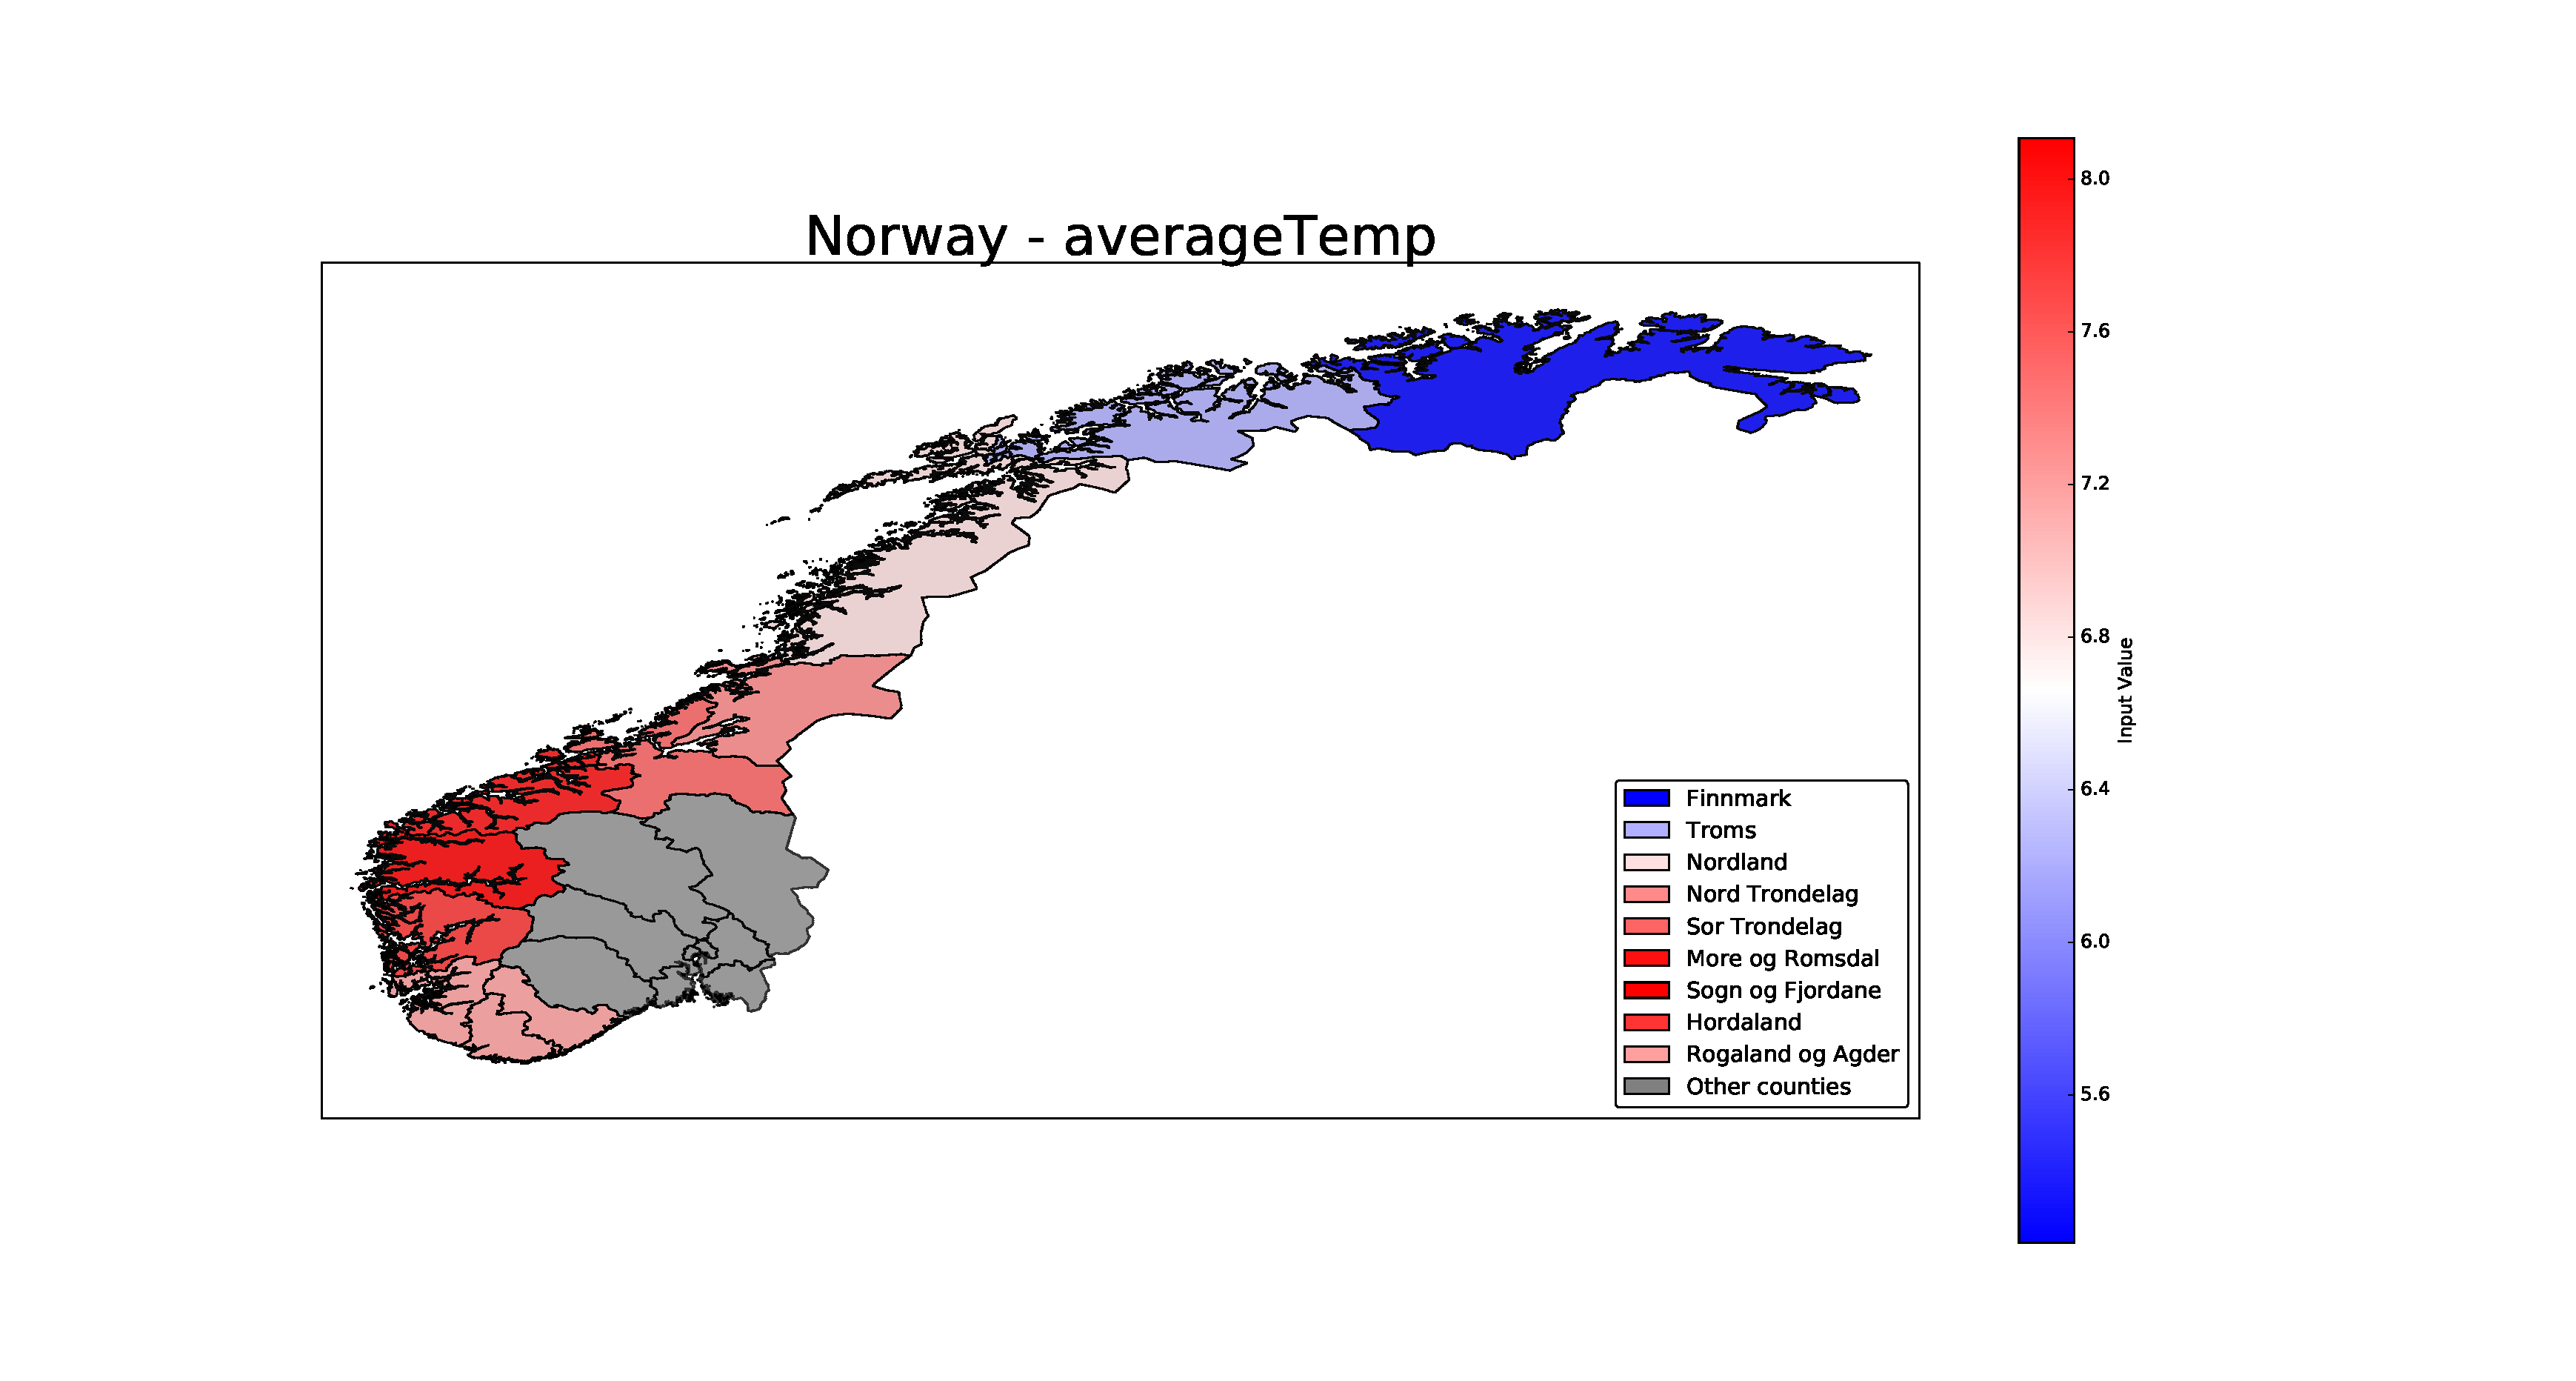
\includegraphics[trim={0cm 2cm 0 3cm},clip, width=1.4\textwidth]{Files/Norway-averageTemp.jpeg}}
    \caption{Average Sea Temperature from 2007 to 2014 in Norway.}
\end{figure}


\chapter{Prediction System}
The main goal during this phase was to find a way to implement a forecast system in Python.
Since the datasets used during this thesis could be considered as a time series, was decide to implement and test an Autoregressive Integrated Moving Average (ARIMA) model. \\
Since there are several possible configurations for fit an ARIMA model, is important to find the right one to use with each input dataset because it would allows to have much better prediction results.
In order to find the best ARIMA configuration there are different methods and procedure, like one of the most known that is "Box–Jenkins method"\footnote{Check out the Box–Jenkins method at the current link: \\ \url{https://en.wikipedia.org/wiki/Box\%E2\%80\%93Jenkins_method}}. In this study was decied to use an easier method, in order to have a first approach with this system and a general idea about the problem. It basically consists in testing different ARIMA model configurations for the same input dataset and then check the results.\\
For this reason during this phase of the work have been implemented 2 different subsytems for two different purposes:
\begin{enumerate}
\item Evaluating System
\item Prediction System
\end{enumerate}

\newpage
\section{Evaluating System}
\textbf{Goal:}\\ 
Used for evaluate different configurations of ARIMA machine. \\ It tests 112 different configurations for the current input that we would like to forecast and report the results with each MAPE (Mean Average Percentage Error) values.

\textbf{Requirements:}\\
There are not any kind of needed requirements. It's possible to use this system on dataset of arbitrary length.

\textbf{Code implementation:}\\
This time the full commented code has not been reported in the appendice since is longer and more complicated than the previous. If you are interested to check out more details about the code, is possible to find the Github repository here : [\ref{Repository}]

The most important part of the code about the Evaluating System is the following.\\
Basically the method ARIMA() allows to train a model based on historic values (history) and a specific order (p,d,q). After that it's possible to call the method forecast() through the trained model and having some predictions like result.
\begin{lstlisting}
model = ARIMA(history, order=arima_order)
model_fit = model.fit(disp=0)
yhat = model_fit.forecast()[0]
\end{lstlisting}

More in the specific, the 112 different ARIMA configurations that were tested are all the possible combinations between the following three parameters values:
\begin{lstlisting}
p_values = [0, 1, 2, 4, 6, 8, 10]
d_values = [0, 1, 2, 3]
q_values = [0, 1, 2, 3]
\end{lstlisting}

\newpage

\textbf{Results:}\\
The system will display the MAPE between real value and predicted values for each of the 112 tested ARIMA machine. In particular, once tested all the configurations, the system will provide the configuration that gave the best MAPE result.\\
All these results have been reported in a document that is possible to check for check out the different configurations result.

The following graphic display the different ARIMA configurations tested, providing also:
\vspace{-5mm}
\begin{itemize}
 \setlength{\itemsep}{-5pt} 
\item General overview about MAPE values for each single tested configuratons. 
\item Best configuration with relative MAPE value.
\item Color legend, where the red means lower MAPE, so more accurate predictions, and blue means higher MAPE, so less accurate predictions.
\end{itemize}

\begin{figure}[H]
	\raggedleft
	\makebox[1\textwidth][c]{\includegraphics[width=1.5\textwidth]{Files/Cages_MAPE.pdf}}
    \caption{Graphic that displays different MAPE values for each ARIMA order.}
\end{figure}

 
 
\newpage
\section{Prediction System}
\textbf{Goal:}\\ 
This system has three main goals:
\vspace{-5mm}
\begin{itemize}
 \setlength{\itemsep}{-5pt} 
\item Testing a specific ARIMA configuration on a particular data input, and display how much accurate it is (MAPE).
\item Predict some future value with the same ARIMA configuration.
\item Display the historic data together with the testing and future predictions.
\end{itemize}

\textbf{Requirements:}\\
There are not any kind of needed requirements. It's possible to use this system on input dataset of arbitrary length.


\textbf{Code implementation:}\\
To reach the first of the goals reported above the system will divide the input dataset in two parts, train and test. It allows to train the ARIMA model with just the "train" part of the dataset, that usually is 66\% of the whole dataset, and then try to predict the rest of the dataset values, comparing in the end with the values contain in the "test" part to have a general idea about the accuracy.

The method ARIMA() allows to train a model based on historic values (history) and a specific order (p,d,q). After that it's possible to call the method forecast() through the trained model and having some predictions like result.

\begin{lstlisting}
model = ARIMA(history, order=arima_order)
model_fit = model.fit(disp=0)
yhat = model_fit.forecast()[0]
\end{lstlisting}

Then the system will also predict a number of future values choosen by the system user.
\begin{lstlisting}
model = ARIMA(dataset, order=order)
model_fit = model.fit(disp=0)
forecast = model_fit.forecast(int(sys.argv[3]))[0]
\end{lstlisting}

The final step is to display the historic data together with the test prediction and the future prediction on the same graphic. 
\begin{lstlisting}
# Plot current input's historic values 
series.plot(color="blue", linewidth=1.5, label="Series: "+sys.argv[1])

# Plot current input's test prediction
predHistoric.plot(color="red", linewidth=1.5, label="Prediction test:")

# Plot current input's future prediction
predFuture.plot(color="green", linewidth=1.5, label="Future Prediction:")
\end{lstlisting}

This time the full commented code has not been reported in the appendice since is longer and more complicated than the previous. If you are interested to check out more details about the code, is possible to find the Github repository here : [\ref{Repository}]

\textbf{Results:}\\
This system will automatically generate two documents that contain:
\vspace{-5mm}
\begin{itemize}
 \setlength{\itemsep}{-5pt} 
\item Test predictions values
\item Future predictions values
\end{itemize}

And then it provides also the possibility to visualize the historic, test and future predictions values on the same graphic, that looks like the following example:

\begin{figure}[H]
    \makebox[\textwidth][c]{\includegraphics[width=1.5\textwidth]{Files/Cages_Predictions.pdf}}
    \caption{Graphic that display historic, future and predicted values of a input.}
\end{figure}


\newpage





\part{Results, Evaluations and Conclusions}

\chap{Results}

The main result of this work is the implemented "Python Analyzer System" itself. It actually provides an automatic way to make an initial analysis and display the results of any input dataset.

Further more has been provided an initial Python implementation of:
\begin{itemize}
\item Future Prediction System
\item Country Map Displaying System
\end{itemize}
\newpage

\begin{figure}[H]
	\centering
    \includegraphics[width=1\textwidth]{Files/Total_Dataset_Matrix.pdf}
    \caption{Correlation matrix between different inputs with data from 2005 to 2016.}
\end{figure}

\begin{table}[ht] 
\makebox[\textwidth][c] {
\resizebox{1.2\textwidth}{!}{\begin{tabular}{ | l | l | l | l | l | l | l | l | l |}
        \hline
INPUTS	& Price 		& Cages 			& Localities		& numberSalmon 		& biomass 		& feedConsumption 		& restock 		& withdrawals 				\\ \hline
Price			& 1			& -0.16		& 0.02 		& 0.52		& 0.51		& 0.28		& 0.11 		& 0.43		\\ \hline
Cages			& -0.16		& 1			& 0.84		& 0.41		& 0.27		& 0.64		& 0.34		& 0.34		\\ \hline
Localities		& 0.02		& 0.84		& 1			& 0.68		& 0.52		& 0.72		& 0.6		& 0.63		\\ \hline
numberSalmon	& 0.52		& 0.41		& 0.68		& 1 		& 0.92		& 0.76		& 0.36		& 0.92		\\ \hline
biomass			& 0.51		& 0.27		& 0.52		& 0.92		& 1			& 0.68		& 0.09		& 0.91		\\ \hline
feedConsumption	& 0.28		& 0.64		& 0.72		& 0.76		& 0.68		& 1			& 0.35		& 0.72		\\ \hline
restock			& 0.11		& 0.34		& 0.6		& 0.36		& 0.09		& 0.35		& 1 		& 0.28		\\ \hline
withdrawals		& 0.43		& 0.34		& 0.63		& 0.92		& 0.91		& 0.72		& 0.28		& 1			\\ \hline
    \end{tabular}}}
    \caption{Dataset inputs correlation coefficients value.}
    \label{table: trendline} 
\end{table}

\newpage

\begin{figure}[H]
	\centering
    \includegraphics[width=1\textwidth]{Files/Norm_Ang_Coeffs.pdf}
    \caption{Normalized angular coefficients of each input's trendline.}
\end{figure}

\begin{table}[ht] 
	\centering
    \begin{tabular}{ | l | l | l | p{5cm} |}
        \hline
        Input 								& Equation 							& Coeff			\\ \hline
          	Salmon\_withdrawals 			& y=464.755139x+(46295.729945) 		& 464.755139 	\\ \hline
          	Salmon\_biomass\_end\_month 	& y=2832.712270x+(354138.727889) 	& 2832.71227 	\\ \hline
          	Salmon\_number\_end\_month 		& y=1543.298421x+(205325.455772)	& 1543.298421 	\\ \hline
          	Salmon\_consumption\_of\_feed 	& y=620.070855x+(58330.012273) 		& 620.070855	\\ \hline
           	Salmon\_price 			& y=0.178175x+(22.643654)			& 0.1781753878 		\\ \hline
          	Salmon\_restock 				& y=89.230600x+(13390.363406)		& 89.2306 		\\ \hline
 			Localities 						& y=0.343533x+(539.979023) 			& 0.343533		\\ \hline
  			Cages 							& y=0.342834x+(3665.904023) 		& 0.342834 		\\ \hline
    \end{tabular} 
    \caption{Dataset inputs trendline equation}
    \label{table: trendline2} 
\end{table}
\begin{table}[ht] 
	\centering
    \begin{tabular}{ | l | l | l | p{5cm} |}
        \hline
        Input 							& Normalized equation 	& Norm Ang Coeffs	\\ \hline
          	Salmon\_withdrawals 		& y=0.003782x+(0.376694)& 0.003782			\\ \hline
          	Salmon\_biomass\_end\_month & y=0.003724x+(0.465599)& 0.003724			\\ \hline
          	Salmon\_number\_end\_month 	& y=0.003639x+(0.484184)& 0.003639			\\ \hline
          	Salmon\_consumption\_of\_feed & y=0.003147x+(0.296085)& 0.003147		\\ \hline
           	Salmon\_price 		& y=0.002625x+(0.333633)
& 0.002625			\\ \hline
          	Salmon\_restock 			& y=0.001217x+(0.182583)& 0.001217			\\ \hline
 			Localities 					& y=0.000531x+(0.834589)& 0.000531			\\ \hline
  			Cages 						& y=0.000082x+(0.877011)& 0.000082			\\ \hline
    \end{tabular} 
    \caption{Dataset inputs normalized trendline equation}
    \label{table: norm_trendline} 
\end{table}

\newpage

\begin{figure}[H]
    \makebox[\textwidth][c]{\includegraphics[width=1.2\textwidth]{Files/Best_MAPE.pdf}}
    \caption{Lower MAPE with best ARIMA Configuration for each tested input.}
\end{figure}

\begin{table}[ht] 
	\centering
    \begin{tabular}{ | l | l | l |}
            \hline
Input							&	ARIMA Conf	&	MAPE	\\ \hline
Cages							&	(10,2,1)	&	1.251\%	\\ \hline
Localities						&	(10,0,1)	&	1.779\%	\\ \hline
Salmon\_price 					&	(0,1,1)		&	6.686\%	\\ \hline
Salmon\_consumption\_of\_feed	&	(6,1,0)		&	6.659\%	\\ \hline
Salmon\_restock 				&	(10,0,1)	&	96.006\%	\\ \hline
Salmon\_withdrawals 			&	(10,0,1)	&	6.277\%	\\ \hline
Salmon\_biomass\_end\_month		&	(8,1,0)		&	1.601\%	\\ \hline
Salmon\_number\_end\_month 		&	(10,2,0)	&	1.723\%	\\ \hline
    \end{tabular}  
    \caption{Best ARIMA configurations with relative MAPE}
    \label{table: Best ARIMA configurations with relative MAPE result in the Evaluation Test} 
\end{table}

\newpage

\makebox[\textwidth][c]{
\resizebox{1.3\textwidth}{!}{
\begin{tabular}{|c|c|c|c|c|c|c|c|c|c|c|c|c|c|}
\hline
\multirow{3}{*}{Months} & \multicolumn{3}{c|}{Cages} & \multicolumn{3}{c|}{Localities} & \multicolumn{3}{c|}{Salmon Biomass} & \multicolumn{3}{c|}{Salmon Number}\\
\cline{2-13}
 & Real & Pred & Error & Real & Pred & Error & Real & Pred & Error & Real & Pred & Error \\
\hline
 January 2017 & 3436 & 3444.87 & 0.26\% & 539.000 & 543.41 & 0.82\% & 738902 & 732841.36 & 0.82\% & 369274 & 366826.189 & 0.66\%\\
\hline
 February 2017 & 3225 & 3251.915 & 0.83\% & 523.000 & 529.05 & 1.16\% & 712981 & 709931.42 & 0.43\% & 347824 & 352905.30 & 1.46\% \\
 \hline
 March 2017 & 3153 & 3164.190 & 0.67\% & 529.000 & 534.29 & 1.00\% & 667749 & 679405.11 & 1.75\% & 343636 & 349747.77 & 1.78\%\\
 \hline
 April 2017 & & 3317.814 & & & 549.14 & & & 657418.41 & & & 369616.83 &  \\
 \hline
 May 2017 & & 3492.701 & & & 550.64 & & & 646850.14 & & & 387244.43 &  \\
 \hline
 June 2017 & & 3507.062 & & & 545.66 & & & 653574.18 & & & 387630.48 & \\
 \hline
 July 2017 & & 3485.804 & & & 560.58 & & & 678469.77 & & & 384314.00 &  \\
 \hline
 August 2017 & & 3588.373 & & & 584.55 & & & 707646.99 & & & 394062.43 & \\
 \hline
 September 2017 & & 3751.633 & & & 596.32 & & & 734628.28 & & & 411164.01 & \\
 \hline
 October 2017 & & 3790.521 & & & 589.11 & & & 757679.66 & & & 411094.09 & \\
 \hline
 November 2017 & & 3710.033 & & & 576.75 & & & 770838.51 & & & 396102.24 & \\
 \hline
 December 2017 & & 3584.505 & & & 563.56 & & & 771279.10 & & & 380399.93 & \\
 \hline
% etc. ...
\end{tabular}  }}


\makebox[\textwidth][c]{
\resizebox{1.3\textwidth}{!}{
\begin{tabular}{|c|c|c|c|c|c|c|c|c|c|c|c|c|c|}
\hline
\multirow{3}{*}{Months} & \multicolumn{3}{c|}{Consumption of feed} & \multicolumn{3}{c|}{Salmon restock} & \multicolumn{3}{c|}{Salmon Withdrawals} & \multicolumn{3}{c|}{Salmon price}\\
\cline{2-13}
 & Real & Pred & Error & Real & Pred & Error & Real & Pred & Error & Real & Pred & Error \\
\hline
 January 2017 & 109341 & 98174.28 & 10.21\% & 4415 & 4734.43 & 7.23\% & 87609 & 90488.98 & 3.29\% & & &\\
\hline
 February 2017 & 88704 & 77998.20 & 12.07\% & 991 & 6904.51 & 596.72\% & 3.29\% & 101295.55 & 11.00\% & & &\\
 \hline
 March 2017 & 87033 & 74726.18 & 14.14\% & 13594 & 15427.63 & 13.49\% & 109498 & 101724.09 & 7.10\% & & &\\
 \hline
 April 2017 & & 88768.11 & & & 39781.36 & & & 95032.95 & & & &\\
 \hline
 May 2017 & & 113280.67 & & & 39438.14 & & & 92065.64 & & & &\\
 \hline
 June 2017 & & 140413.56 & & & 22562.89 & & & 88775.54 & & & &\\
 \hline
 July 2017 & & 164511.15 & & & 20449.85 & & & 92643.44 & & & &\\
 \hline
 August 2017 & & 179690.48 & & & 39487.67 & & & 104102.60 & & & &\\
 \hline
 September 2017 & & 181556.12 & & & 49991.91 & & & 110419.37 & & & &\\
 \hline
 October 2017 & & 169502.10 & & & 31449.69 & & & 107588.69 & & & &\\
 \hline
 November 2017 & & 147770.73 & & & 11698.23 & & & 102943.86 & & & &\\
 \hline
 December 2017 & & 123447.55 & & & 7957.45 & & & 99561.98 & & & &\\
 \hline
% etc. ...
\end{tabular}  }}


 % Results
\chap{Discussion and Extended Evaluations}

The current study investigates the possibility of testing the Data Science process using Python, trying to apply it to the Norwegian salmon farming industry, in order to gather and let be available as many useful results as possible.

\section{Evaluations of the study}
During this work is shown that is actually possible to have a first approach to the Data Science field using Python. All the documented steps of this works allow to have a complete overview of the general Data Science process.

Furthermore, the resulting Python systems and the corresponding evidences are showing which modules and packages are provided by Python in order to analyze, display and forecast data values. The high reusability and automation levels of the implemented system allow to easily reuse it in order to apply the same analysis, displaying and forecasting on a different dataset that contains data from a different area of interest. \\
On the other side the current system is probably efficient and productive for a personal use. That's because is not provided an implemented GUI, and to customize the system's outputs you have to have some basic knowledge of Python language, that could be a limitation for several people, but it could also be considered like an incentive for people to get to know this powerful programming language.

The approach used for this thesis didn't provide any kind of results that can be considered as new information about the Norwegian salmon farming field, but it provided a new way to visualize large amounts of data and also several discussion's starting points for further works. That's because this thesis was mainly focused on the Data Science process, Python utilities and to find out observations for future researches instead of the information extraction process itself.

Even that, as reported in the Results Overview chapter, several systems, evidences and values have been calculated and reported during this work. 

In the next sections are reported the discussions that I considered most relevant and interesting for further works, and then are reported the encountered limitations. 

\section{Considerations about implemented Evaluation System }
\label{Discussion1}
The following resulting table reveals several informations. \\
The column "Evaluation MAPE" is the average MAPE of the forecasted values during the Evaluation System with the reported ARIMA order. \\ 
The column "Forecast MAPE" represents the average MAPE of the 12 values predicted in the future, already reported in the results. [\ref{table: RealPredMAPE1}] 

 \begin{table}[ht]
\makebox[1\textwidth][c]{
    \begin{tabular}{ | l | l | l | l | l |}
            \hline
\textbf{County} 	& \textbf{Parameter} & \textbf{ARIMA Order}	& \textbf{Evaluation MAPE} 	& \textbf{Forecast MAPE} 	\\ \hline
Finnmark 	& feedConsumption				& (6, 1, 0) 			& 13.771\% 	&	19.20\% 		\\ \hline	
Hordaland 	& feedConsumption				& (8, 0, 0)  			& 6.811\%	& 	17.89\%			\\ \hline				
Troms 		& feedConsumption				& (2, 0, 0)  			& 11.593\% 	&	43.04\%			\\ \hline
Nordland 	& feedConsumption				& (6, 0, 0)  			& 12.741\%	&	26.01\% 		\\ \hline
Norway0714 	& feedConsumption				& (6, 1, 0)  			& 7.296\%  	&	7.94\%			\\ \hline
    \end{tabular}}
         \caption{Comparison between Evaluation MAPE and Prediction MAPE}   
   \label{table: MAPE_Comparison} 
\end{table}        

From the values contained in the table [\ref{table: MAPE_Comparison}] is possible to see that the average MAPE for the forecasted future values (\textbf{Forecast MAPE}) is much higher than the one reported from the evaluation process (\textbf{Evaluation MAPE}) . \\
There is just one particular case where the Evaluation MAPE and Forecast MAPE values are really close, that is the one about the Norway dataset.

At this point, it would be extremely useful to discover why the predicted future values about the dataset 'Norway0714' are much more accurate and why their average MAPE is really close to the one calculated during the evaluation procedure.\\
In order to understand the reason, certain analysis through the resulting evidences have been made. Below here are reported the considerations about it:
\vspace{-5mm}
\begin{itemize}
 \item Checked the annual feed consumption trend during different years for the current datasets, that is possible to check out in the reported graphics [\ref{fig: Norway_feed}]. No big differences between the Norway's trend compared with the others was found.
 \item Checked correlation coefficients between different years of the feed consumption values for each tested dataset, but there were not any kind of significant high/low correlation levels with the years before.
 \item Tried to execute the prediction system with settings that are different by the one suggested in the Evaluation system results. Found that for some particular dataset is possible to get better predictions with a different configuration, like for example: \\
 Prediction system about "feed consumption" in Nordland executed with the suggested configuration (6,0,0) shows an average MAPE value equal to 26.01\% for the predicted values. If the Prediction system is tested on the same input but fitting the ARIMA model with the order (6,1,0) the average MAPE value decrease to 16.82\% for the predicted values. It's possible to clearly see this difference watching at the graphics reported in the following page: [\ref{fig: Nordland_ARIMAevaluation}] and [\ref{fig: Nordland_ARIMAmanual}]. \\ 
Furthermore, it's possible to check in the table [\ref{table: MAPE_Comparison}] that the configuration of Troms gives the worst Evaluation MAPE result, and once tested with a manual configuration of (6, 1, 0) the resulting MAPE is decrease to 21.05\%.
\end{itemize}

This shows that the initial Evaluation system is not that accurate and reliable for each kind of input dataset. For this reason, in order to improve it during further works, is strongly suggest to try the "Box-Jenkinks method" for determine the best ARIMA order's parameters, that would probably be better and more specific for each single dataset. It provides a more accurate procedure for analyze a series, in order to determine the best ARIMA parameters to use. More details about it are reported in recommendation for further works.


\newpage

\begin{figure}[H]
	\makebox[\textwidth][c]{
    \includegraphics[trim={0 1cm 0 0},clip,width=1.3\textwidth]{Files/Nordland-feedConsumption_pred.pdf}}
    \caption[Predicted 2015 feed consumption in Nordland. Evaluation system ARIMA order.]{Predictions of 2015 feed consumption values in Nordland using ARIMA model fitted with the order suggested by the evaluation system results (6,0,0).\\  It provides an average MAPE of 26.01\% between the real and predicted 2015 values. }
    \label{fig: Nordland_ARIMAevaluation}
\end{figure}

\begin{figure}[H]
	\makebox[\textwidth][c]{
    \includegraphics[trim={0 1cm 0 0},clip,width=1.3\textwidth]{Files/Nordland-feedConsumption_BETTER.pdf}}
    \caption[Predicted 2015 feed consumption in Nordland. Manual ARIMA order.]{Predictions of 2015 feed consumption values in Nordland using ARIMA model fitted with an order manually chosen (6,1,0).\\  It provides an average MAPE of 16.82\% between the real and predicted 2015 values. }
    \label{fig: Nordland_ARIMAmanual}
\end{figure}


\newpage

\section{Extended evaluations: feed consumption forecasting }
\label{Discussion2}
During the implementation of this work, was also noticed a strong relation between the two parameters "Sea Average Temperature" and "Feed Consumption".
I decided to focus on this particular correlation because, also if it's already well known that is possible to feed more the salmon when the temperature is higher, it could be very useful for further predictions about feed consumption values, since the sea average temperature would be considered like a parameter to use for improve the final results.

This correlation is significant for all the Norwegian counties and it's clearly possible to see it with the example graphic\footnote{The graphics reported above have been displayed with a Python system implemented during this study, that allows to display different parameters in a normalized range. The system has not been reported in the thesis work, but is possible to find it here named "Analysis.py": \\ \url{https://github.com/Sprea22/Personal_Utilities}} reported below here. 

\vspace{-10mm}

\makebox[1\textwidth][c]{
\begin{minipage}[t]{0.6\textwidth}
\begin{figure}[H]
    \includegraphics[trim={0 0.5cm 0 0},clip,width=1\textwidth]{Files/Finnmark-Temp&Feed.png}
    \caption[Finnmark: average sea temperature compared with feed consumption]{Comparison between average sea temperature and feed consumption in Finnmark}
    \label{fig: Finnmark_seaTemp&feed}
\end{figure}
\end{minipage} \hfill
\begin{minipage}[t]{0.6\textwidth}
\begin{figure}[H]
	\centering
    \includegraphics[trim={0 0.5cm 0 0},clip,width=1\textwidth]{Files/Troms-Temp&Feed.png}
    \caption[Troms: average sea temperature compared with feed consumption]{Comparison between average sea temperature and feed consumption in Troms}
    \label{fig: Troms_seaTemp&feed}
\end{figure}
\end{minipage}}
\makebox[1\textwidth][c]{
\begin{minipage}[t]{0.6\textwidth}
\begin{figure}[H]
    \includegraphics[trim={0 0.5cm 0 1cm},clip,width=1\textwidth]{Files/Nordland-Temp&Feed.png}
    \caption[Nordland: average sea temperature compared with feed consumption]{Comparison betwen average sea temperature and feed consumption in Nordland}
    \label{fig: Nordland_seaTemp&feed}
\end{figure}
\end{minipage} \hfill
\begin{minipage}[t]{0.6\textwidth}
\begin{figure}[H]
	\centering
    \includegraphics[trim={0 0.5cm 0 1cm},clip,width=1\textwidth]{Files/Hordaland-Temp&Feed.png}
    \caption[Hordaland: average sea temperature compared with feed consumption]{Comparison between average sea temperature and feed consumption in Hordaland}
    \label{fig: Hordaland_seaTemp&feed}
\end{figure}
\end{minipage}}

\newpage

The following graphics allow to have a very clear overview of what just written above.\\
\vspace{-10mm}
\begin{itemize}
 \setlength{\itemsep}{-5pt}
 \item In the first graphic the average sea temperature (Celsius) is reported , where blue means lower temperature and red higher temperature.
 \item In the second graphic the feed consumption per biomass (kg/kg) is reported , where red means an higher consumption and blue a lower one.
\end{itemize}

So it's clearly possible to see how the average sea temperature and the feed consumption per biomass have a significant correlation for every single Norwegian county.

\begin{figure}[H]
	\makebox[\textwidth][c]{
    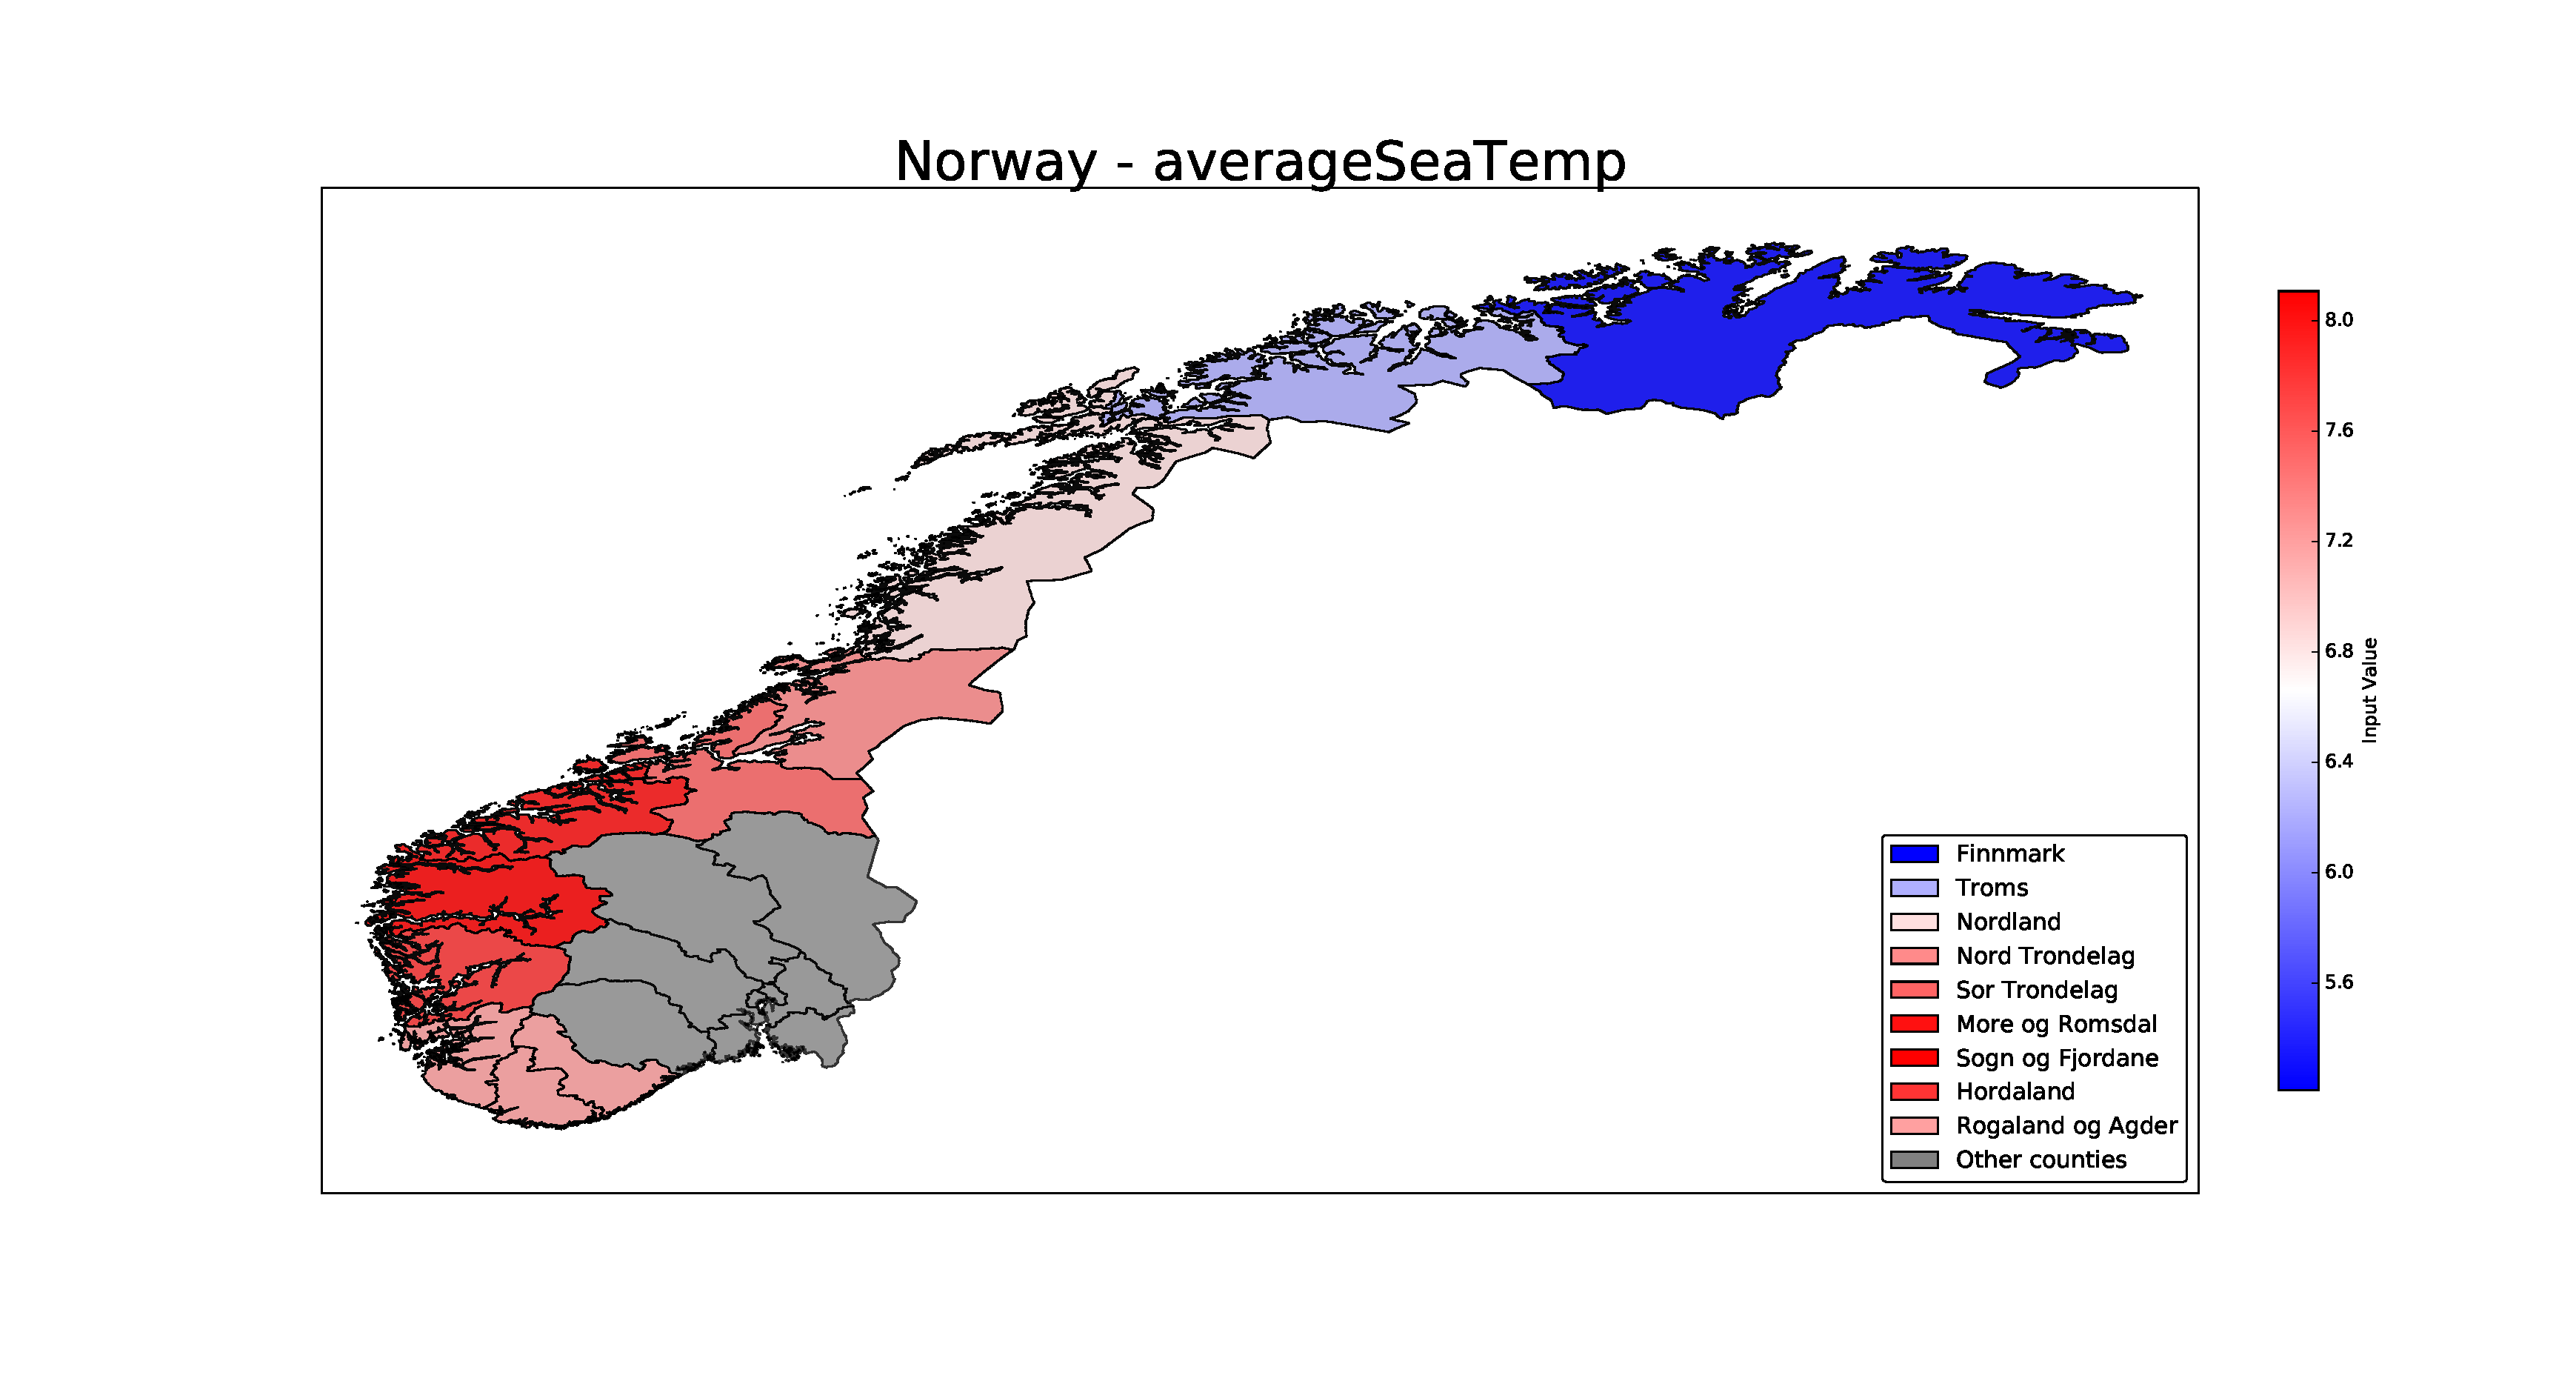
\includegraphics[trim={0 4cm 0 3cm},clip,width=1.3\textwidth]{Files/norway_averageSeaTemp.pdf}}
    \caption{Shows the average of the monthly average sea temperature (Celsius) from 2007 to 2014 in Norway}
    \label{fig: Norway_averageSeaTemp}
\end{figure}

\begin{figure}[H]
	\makebox[\textwidth][c]{
    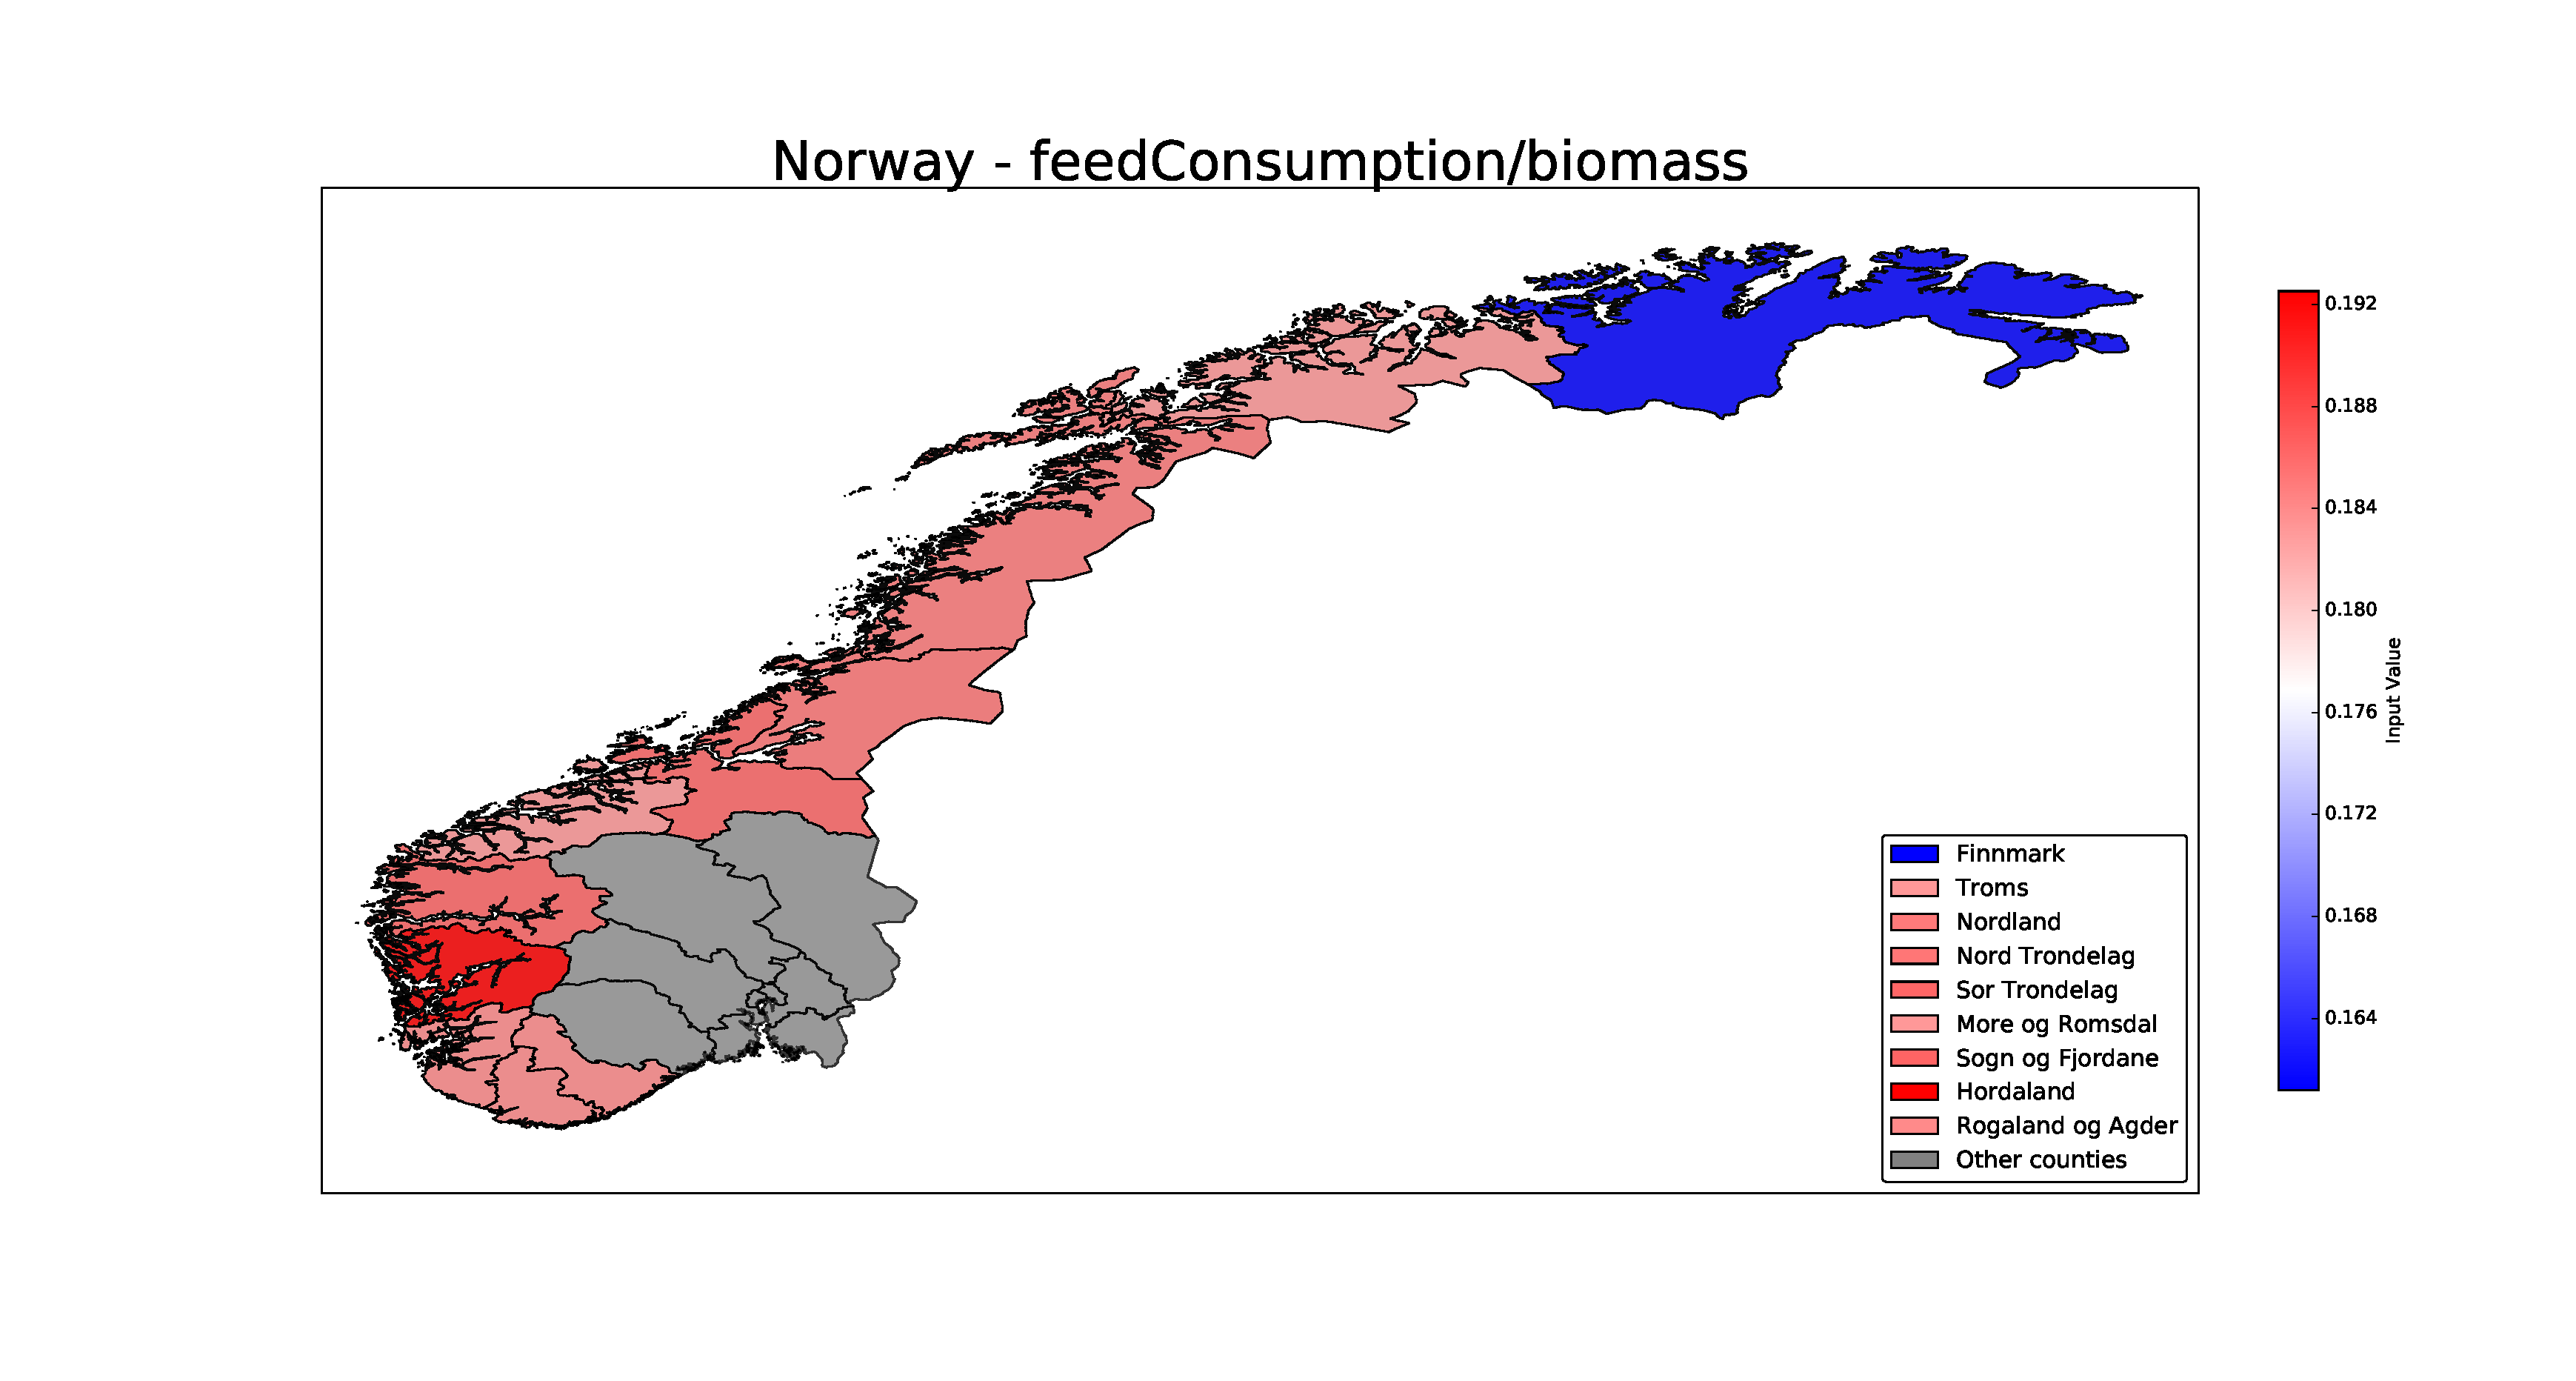
\includegraphics[trim={0 4cm 0 3cm},clip,width=1.3\textwidth]{Files/norway_feed-biomass.pdf}}
    \caption{Shows the average of the monthly average feed consumption per biomass (kg/kg)from 2007 to 2014 in Norway}
    \label{fig: Norway_feed-biomass}
\end{figure}

\newpage

Furthermore, it is even possible to check the correlation coefficient values reported in the correlation matrix below here. These graphic represent the correlation coefficient between different parameter about the same dataset (county in this case).\\
You can find the the correlation coefficient value's representation at the crossing point between "averageSeaTemp" and "FeedConsumption" of each correlation matrix represented below here.\\
It's possible to see that the correlation value's representation shows an high correlation value (red means high correlation) between the two parameters. Even if you check through the other Norwegian counties correlation matrix, this high correlation is valid.\\


  \vspace{-10mm}
  
\makebox[1\textwidth][c]{
\begin{minipage}[t]{0.6\textwidth}
\begin{figure}[H]
    \includegraphics[trim={0 0 0 0},clip,width=1\textwidth]{Files/Finnmark_Total_Matrix.pdf}
    \caption[Correlation matrix between parameter of Finnmark dataset.]{Correlation matrix between all the parameters of the dataset about Finnmark}
    \label{fig: Finnmark_parametersComparison}
\end{figure}
\end{minipage} \hfill
\begin{minipage}[t]{0.6\textwidth}
\begin{figure}[H]
	\centering
    \includegraphics[trim={0 0 0 0},clip,width=1\textwidth]{Files/Troms_Total_Matrix.pdf}
    \caption[Correlation matrix between parameter of Troms dataset.]{Correlation matrix between all the parameters of the dataset about Troms}
    \label{fig: Troms_parametersComparison}
\end{figure}
\end{minipage}}
\makebox[1\textwidth][c]{
\begin{minipage}[t]{0.6\textwidth}
\begin{figure}[H]
    \includegraphics[trim={0 0 0 0},clip,width=1\textwidth]{Files/Nordland_Total_Matrix.pdf}
    \caption[Correlation matrix between parameter of Nordland dataset.]{Correlation matrix between all the parameters of the dataset about Nordland}
    \label{fig: Nordland_parametersComparison}
\end{figure}
\end{minipage} \hfill
\begin{minipage}[t]{0.6\textwidth}
\begin{figure}[H]
	\centering
    \includegraphics[trim={0 0 0 0},clip,width=1\textwidth]{Files/Hordaland_Total_Matrix.pdf}
    \caption[Correlation matrix between parameter of Hordaland dataset.]{Correlation matrix between all the parameters of the dataset about Hordaland}
    \label{fig: Hordaland_parametersComparison}
\end{figure}
\end{minipage}}


\section{Limitations of the study}
\vspace{-5mm}
This study has a number of limitations, mainly due to:
\vspace{-5mm}
\begin{itemize}
 \setlength{\itemsep}{-5pt}
  \item Hard to get access to salmon farming knowledge.
  \item Relatively short time available for this work since data time takes time.
\end{itemize}

As Senior Editor Amanda Hindle wrote, "No one expects science to be perfect the first time and while your peers can be highly critical, no one’s work is beyond limitations. Our knowledge base is built on uncovering each piece of the puzzle, one at a time, and limitations show us where new efforts need to be made. So much like peer review, don’t think of limitations as being inherently bad, but more an opportunity for a new challenge. In the end, your limitation may be someone else’s inspiration." \cite{limitations}

During this work I got more and more knowledge and experience mainly about the fields (Data Science procedures and Salmon farming in Norway), and it allowed to get anyway some positive and useful results that provide an answer to most of the initial objectives of this thesis. \\
  
 % Evaluations
\chap{Conclusion}

\section{Summary}

This study was mainly focused on having an initial approach with Data Science field, in order to investigate and document possible methods and techniques for visualization and prediction of data. At the same time, another goal of this work was to evaluate the feasibility of Python in Data Science, describing implementation procedures and reporting observations.
Specifically, a Python procedure was applied for reporting the initial analysis, displaying and forecasting results about Norwegian salmon farming, in order to provide structured, described and accessible data.

This study concludes that Python has a significant potential in the Data Science field. \\ In particular, the implemented procedure is reporting and describing the main Python modules and packages that can be used for analysis, displaying and forecasting of data. This procedure also provides a general idea about a forecasting system, showing the main problems, challenges and reporting possible methods that can be used for improve its implementation. 
Last but not least, this thesis introduces some significant discussion points, particularly about forecasting evaluation system improvements [\ref{Discussion1}] and feed consumption predictions [\ref{Discussion2}], that are providing useful suggestions and ideas for further works, which are even reported in the next section [\ref{Recommendations}].

\newpage
\section{Recommendations to future work}
\label{Recommendations}
\vspace{-5mm}
In this section are reported some ideas for future work and some extra implementation that have not been implemented during this thesis due to the time limitation. Some of them could be considered interesting for future reserach or analysis.
\begin{itemize}
\item \textbf{Improve the dataset content}\\ The data collection that has done during this thesis provides just public data about territorial statistics. Would be interesting to test the same system with data coming from single reality, like for example in this case gather data from a single locality of salmon farming and then run the system on it.
\item \textbf{Visualization of the data}\\ Also if the library used during this study allow a quite good visualization of the data, it would be useful to check out other ways to realize it, which could imply the use of Python or not. For instance, if you still want to use Python could be possible to check out other libraries, such as "Plotly Python Library"\footnote{Link to Plotly Library : \url{https://plot.ly/python/}}.
\item \textbf{System as a service}\\ Would be really interesting to investigate about a possible way to provide this kind of analysis, displaying and forecasting systems like a service, such as this following simple idea:\\

\begin{figure}[H]
	\centering
       \makebox[1\textwidth][c]{\includegraphics[width=0.8\textwidth]{Files/ServiceSystem.pdf}}
    \caption{General idea about Prediction Systems as a service.}
\end{figure}

\newpage

\item \textbf{Improve the ARIMA evaluation system}\\ Since the Evaluation system implemented during system was a very basic and easy implementation, I strongly recommend to check out the "Box–Jenkins method"\cite{wiki:BoxJenkinsMethod}. In time series analysis this method applies autoregressive integrated moving average (ARIMA) models to find the best fit of a time-series model to past values of a time series. It provide a three phase approach, that are model identification, parameter estimation and model checking. In particular, it provides a clear description of how to interpret the graphic, such as the autocorrelation plot of a series, that is very important for identify stationarity and seasonality of a series, which are indispensable details to consider if you want to improve the prediction system.

\item \textbf{Improve the prediction system}\\ This is the part which has much more possible future works. Forecasting system development is today a fundamental issue that involves different area of studies. To achieve an accurate model and significant results it needs much more specific research than the one reported in this study, that was just for report a general idea about it. I strongly recommend for further works:
\begin{itemize}
\item Improve this forecasting model, applying and studying the "Box-Jenkins method"\footnote{Box-Jenkins method : \url{https://en.wikipedia.org/wiki/Box\%E2\%80\%93Jenkins\_method}} in order to improve the Evaluation system and get better predictions of future value.z
\item If you are interested in "salmon feed consumption" forecasting I strongly suggest you to consider the discussion about the relation between "Feed Consumption" and "Average Sea Temperature", since it could provides a significant help in order to improve the accuracy level of the system.
\end{itemize}
\end{itemize}


\addtocontents{toc}{\vspace{\normalbaselineskip}}

 % Conclusion

%\input{Chapters/Future_Works}


%% Appendices -----------------------------------------------------



\addtocontents{toc}{\vspace{2em}} % Add a gap in the Contents, for aesthetics

\lhead{\emph{Appendices}}  % Change the left side page header to "Appendices"

\part{Code Full Implementation}
\begin{appendix}

\chap{SIA Implementation code}
\label{SIA_Implementation}

\section{SIA: Imported libraries}
\label{SIA_libraries}
The library "os" is really important since provides a waay of using operating system dependent functinality.
\begin{lstlisting}
import os
\end{lstlisting}

Also the library "sys" would be very useful for test and execute the program, mainly because it allows to input directly from terminal.
\begin{lstlisting}
import sys
\end{lstlisting}

The "pylab" library will be useful for plot data.
\begin{lstlisting}
import pylab
\end{lstlisting}

The "pandas" library will be very useful for read the data from CSV dataset and setup the plot abut it.
\begin{lstlisting}
import pandas as pd
\end{lstlisting}

The "numpy" library it's used for mathematic purpose, such as calculating the correlation coefficent between two series.
\begin{lstlisting}
import numpy as np
\end{lstlisting}
 
The "pyplot" library it's used for basic graphic displaying and customization, easy to use but very efficent.
\begin{lstlisting}
import matplotlib.pyplot as pyplot
\end{lstlisting}

The library "PIL" supports many file formats, and provides powerful image processing and graphics capabilities.
\begin{lstlisting}
from PIL import Image
\end{lstlisting}

The library "fpdf" allows to generate and use PDF file.
\begin{lstlisting}
from fpdf import FPDF
\end{lstlisting}

\section{SIA section I: Total graphic for all the years}
\label{SIA_section_I}
\textbf{Code implementation:}\\
During this section of the code was used "pandas" library for read the dataset.
\begin{lstlisting}
series = pd.read_csv("Dataset.csv", usecols=[1,sys.argv[1]])
\end{lstlisting}

Then using the "pyplot" library has been possible to setup the plot of the input data.
\begin{lstlisting}
series.plot(color="blue", linewidth=1.5)
\end{lstlisting}


Thera are some settings about the axis x just to display the data in the right format, are easy to change and to costume.
\begin{lstlisting}
years = ["2005","2006","2007","2008","2009","2010",
	"2011","2012","2013","2014","2015","2016"]
x = range(144)
pyplot.xticks(np.arange(min(x), max(x)+1, 12.0), years)
pyplot.title("Total graphic from 2005 to 2016")
\end{lstlisting}

Once setted up the plot of the current data, the next step was to display the trendline of the current graphic. \\ 
The following code represent the method for calculate and display it.
\begin{lstlisting}
def trendline(x, y, col):
	z = np.polyfit(x, y, 1)
	p = np.poly1d(z)
	pylab.plot(x,p(x), c=col)
	# print "y=%.6fx+(%.6f)"%(z[0],z[1])
\end{lstlisting}	

At this point the current data values have been read again and passed to the method just impleneted above for calculating the trendline.
\begin{lstlisting}
series2 = pd.read_csv("Dataset.csv", usecols=[sys.argv[1]],
			squeeze=True)
trendline(x, seriesV.values, "red")
\end{lstlisting}

There is the possibility to save the graphic like an image and/or display it.
\begin{lstlisting}
saveFigure("_Total.jpg")
\end{lstlisting}


\section{SIA section II: Single graphics for each year}
\label{SIA_section_II}
\textbf{Code implementation:}\\
During this section of the code was used "pandas" library for read the dataset.
\begin{lstlisting}
series2 = pd.read_csv("Dataset.csv", index_col=['Month'],
			usecols=[0,1,sys.argv[1]])
\end{lstlisting}

Some initialization of variables that are going to be useful.
\begin{lstlisting}
months = ["Jan","Feb","Mar","Apr","May","Jun",
		"Jul","Aug","Sep","Oct","Nov","Dec"]
x_pos = np.arange(len(months))
test = []
j = 0
\end{lstlisting}

The following code allows the system to split the values and display them in the right way: that means that are going to be splitted for each single year and then plotted on the same graphic.
\begin{lstlisting}
for i in range(len(series2.values)):
	if j in range(12):
		test.append(series2.values[i][1])
		j = j + 1
	else:
		pyplot.plot(x_pos, test, linewidth=2, 
			alpha=0.8, 
			label = int(series2.values[i-1][0]))
		test = []
		test.append(series2.values[i][1])
		j = 1

\end{lstlisting}

These are some personalization settings that could be easily changed as you want.
\begin{lstlisting}
ax.legend(loc=4, ncol=1, fancybox=True, shadow=True)
pyplot.xticks(x_pos,months)
pyplot.xlim(0,11)
pyplot.title(sys.argv[1]+ 
		": Single year's graphic from 2005 to 2016")
\end{lstlisting}

There is the possibility to save the graphic like an image and/or display it.
\begin{lstlisting}
saveFigure("_Years.jpg")
\end{lstlisting}


\section{SIA section III: Correlation matrix between years}
\label{SIA_section_III}
\textbf{Code implementation:}\\
During this section of the code was used "pandas" library for read the dataset.
\begin{lstlisting}
series3 = pd.read_csv("Dataset.csv", index_col=['Year'],
			usecols=[0,sys.argv[1]])
\end{lstlisting}

\begin{lstlisting}
corr = []
test = []
j = 0
# Collecting the correct values to elaborate.
for i in range(len(series2.values)+1):
	if j in range(12):
		test.append(series2.values[i][1])
		j = j + 1
	else:
		corr.append(test)
		test = []
		if i in range(144):
			test.append(series2.values[i][1])
			j = 1
\end{lstlisting}

With the library "numpy" is possible to calculate the correlation coefficents between all the variables in the series just read.
\begin{lstlisting}
test = np.corrcoef(corr)
\end{lstlisting}

Setup the figure that will display the correlation matrix using the library "pypot".
\begin{lstlisting}
fig2 = pyplot.figure()
ax = fig2.add_subplot(111)
\end{lstlisting}

Creating the correlation matrix using the already calculated correlation coefficents.
\begin{lstlisting}
cax = ax.matshow(test, interpolation='nearest')
\end{lstlisting}

Settings for display the matrix in the right way, in particular for the values to display on both the axis x and y, in this case every single year from 2005 to 2016
\begin{lstlisting}
pyplot.title(sys.argv[1]+ ": Correlation between different years")
years = ["2005","2006","2007","2008","2009","2010",
	"2011","2012","2013","2014","2015","2016"]
x_pos = np.arange(len(years))
y_pos = np.arange(len(years))
pyplot.yticks(y_pos,years)
pyplot.xticks(x_pos,years)
pyplot.colorbar(cax)
\end{lstlisting}
\newpage
Adding a title to the graphic that we are going to display and also a bar that works like a legend for the colors of the matrix, allowing the reader to better understand the values reported inside the matrix.
\begin{lstlisting}
saveFigure("_Years_Matrix.jpg")
\end{lstlisting}

There is the possibility to save the correlation matrix like an image and/or display it.
\begin{lstlisting}
pyplot.savefig("OUTPUT_DIRECTORY", format="jpg")
pyplot.show()
\end{lstlisting}


\section{SIA section IV: Correlation matrix between months}
\label{SIA_section_IV}
\textbf{Code implementation:}\\
During this section of the code was used "pandas" library for read the dataset.
\begin{lstlisting}
series4 = pd.read_csv("Dataset.csv", usecols=[0,1,sys.argv[1]])
\end{lstlisting}

\begin{lstlisting}
corr = []
for Month, Year in series4.groupby(["Month"], sort=False):
	corr.append(Year[sys.argv[1]].values)
\end{lstlisting}
	
With the library "numpy" is possible to calculate the correlation coefficents between all the variables in the series just read.
\begin{lstlisting}
test = np.corrcoef(series4.values)
\end{lstlisting}

Setup the figure that will display the correlation matrix using the library "pypot".
\begin{lstlisting}
fig2 = pyplot.figure()
ax = fig2.add_subplot(111)
\end{lstlisting}

Creating the correlation matrix using the already calculated correlation coefficents.
\begin{lstlisting}
cax = ax.matshow(test, interpolation='nearest')
\end{lstlisting}

Settings for display the matrix in the right way, in particular for the values to display on both the axis x and y, in this case every single months of the year.
\begin{lstlisting}
months = ["Jan","Feb","Mar","Apr","May","Jun",
	"Jul","Aug","Sep","Oct","Nov","Dec"]
x_pos = np.arange(len(months))
y_pos = np.arange(len(months))
pyplot.yticks(y_pos,months)
pyplot.xticks(x_pos,months)
\end{lstlisting}
Adding a title to the graphic that we are going to display and also a bar that works like a legend for the colors of the matrix, allowing the reader to better understand the values reported inside the matrix.
\begin{lstlisting}
pyplot.title("Correlation between different months")
pyplot.colorbar(cax)
\end{lstlisting}

There is the possibility to save the correlation matrix like an image and/or display it.
\begin{lstlisting}
saveFigure("_Months_Matrix.jpg")
pyplot.show()
\end{lstlisting}

\section{SIA section V: Single overview}
\label{SIA_section_V}
\textbf{Code implementation:}\\
create\_single\_overview() : this method will use the "Image" library for autogenerate a collage of the current input's graphics and save it like an overview image. The content of the params will basically decide how the "Current input overview image" will looks like.

It uses each single "current input overview image" of all the inputs and the "correlation matrix between all the inputs image" for combine them in a unique "total overview" and save it using the PDF format.

\begin{lstlisting}
listofimages=["CURRENT_INPUT_TOTAL_GRAPHIC",
            "CURRENT_INPUT_YEARS_MATRIX", 
            "CURRENT_INPUT_YEARS_GRAPHIC",
            "CURRENT_INPUT_MONTHS_MATRIX"]
            
create_single_overview(params1, listofimages)
create_single_overview(params2, listofimages)
\end{lstlisting}


The "create\_single\_overview" method has basically this structured, and then its configuration depends from the input data and from the preferences.
\begin{lstlisting}
def create_single_overview(cols, rows ,
			width, height, listofimages):
    thumbnail_width = width//cols
    thumbnail_height = height//rows
    size = thumbnail_width, thumbnail_height
    new_im = Image.new('RGB', (width, height))
    ims = []
    for p in listofimages:
        im = Image.open(p)
        im.thumbnail(size)
        ims.append(im)
    i = 0
    x = 0
    y = 0
    for col in range(cols):
        for row in range(rows):
            new_im.paste(ims[i], (x, y))
            i += 1
            y += thumbnail_height
        x += thumbnail_width
        y = 0
    new_im.save(SINGLE_OVERVIEW_IMAGE")
	new_im.show()
\end{lstlisting}
 % SIA Implementation code

\chap{MIA Implementation code}

\section{MIA: Imported libraries}
The "pandas" library will be very useful for read the data from CSV dataset and setup the plot abut it.
\begin{lstlisting}
import pandas as pd
\end{lstlisting}

The "numpy" library it's used for mathematic purpose, such as calculating the correlation coefficent between two series.
\begin{lstlisting}
import numpy as np
\end{lstlisting}

 
The "pyplot" library it's used for basic graphic displaying and customization, easy to use but very efficent.
\begin{lstlisting}
import matplotlib.pyplot as pyplot
\end{lstlisting}

\section{MIA: Implementation}
\textbf{Code implementation:}\\
First of all, we are going to use the "pandas" library for read the dataset.
\begin{lstlisting}
series3 = pd.read_csv("TOTAL_DATASET_DIRECTORY", 
	index_col=['Input'], header=0)
\end{lstlisting}

Then with the library "numpy" is possible to calculate the correlation coefficents between all the variables just read above.
\begin{lstlisting}
test = np.corrcoef(series3.values)
\end{lstlisting}

Setup the figure that will display the correlation matrix using the library "pyplot".
\begin{lstlisting}
fig2 = pyplot.figure()
ax = fig2.add_subplot(111)
\end{lstlisting}

Creating the correlationg matrix using the already calculated correlation coefficents.
\begin{lstlisting}
cax = ax.matshow(test, interpolation='nearest')
\end{lstlisting}

Settings for display the matrix in the right way, in particular for the values to display on both the axis x and y, in this case every single input.
\begin{lstlisting}
inputs = ["Cages", "Feed", "Number", "Restock",
	"Local", "Withdr", "Biomass", "Price"]
x_pos = np.arange(len(inputs))
y_pos = np.arange(len(inputs))
pyplot.yticks(y_pos,inputs)
pyplot.xticks(x_pos,inputs)
\end{lstlisting}

Adding a title to the graphic that we are going to display and also a ba that works like a legend for the colors of the matrix, allowing the reader to better understand the values reported inside the matrix.
\begin{lstlisting}
pyplot.title("Correlation between different inputs 
		about data from 2005 to 2016")
pyplot.colorbar(cax)
\end{lstlisting}

In the end, using again the library "pyplot", there is the possibility to save the correlation matrix graphic like an image and/or display it.
\begin{lstlisting}
pyplot.savefig("OUTPUT_DIRECTORY")
\end{lstlisting}

\begin{lstlisting}
series = pd.read_csv("TRENDLINES_VALUES_DOCUMENT",
	 header=0, usecols=["Norm Ang Coeffs"])
series.plot(kind="barh")
pyplot.savefig("OUTPUT_DIRECTORY")

create_total_overview()
\end{lstlisting}

\begin{lstlisting}
pyplot.show()
\end{lstlisting}

 % MIA Implementation code

\chapter{Norway's Map System Implementation Code}
\label{MapNOR}
\begin{lstlisting}
import os
import sys
import matplotlib
import pandas as pd
import cartopy.crs as ccrs
import matplotlib.cm as cmx
import matplotlib.pyplot as plt
import matplotlib.patches as mpatches
import cartopy.io.shapereader as shpreader
\end{lstlisting}

\begin{lstlisting}
def add_geom(axes, shapeInput, labelInput, colorInput):
	axes.add_geometries(shapeInput, ccrs.Robinson(), edgecolor='black',label = labelInput, facecolor=colorInput, alpha=0.8)
	return mpatches.Rectangle((0, 0), 1, 1, facecolor=colorInput)
\end{lstlisting}

\begin{lstlisting}
def main():
# Downloaded from http://biogeo.ucdavis.edu/data/gadm2.8/shp/NOR_adm_shp.zip
	fname = 'Datasets/NOR/NOR_adm1.shp'
	NOR_shapes = list(shpreader.Reader(fname).geometries())
	plt.figure()
	ax = plt.axes(projection=ccrs.Robinson())
	ax.coastlines(resolution='10m')
	ax.set_extent([4, 32, 57, 72], ccrs.Robinson())	

	colMap='bwr'
	dataInput = sys.argv[1]
	inputSeries = pd.read_csv("Datasets/countiesAverages.csv")

	inputValues = [inputSeries[dataInput][0], inputSeries[dataInput][1], inputSeries[dataInput][2], inputSeries[dataInput][3],
	inputSeries[dataInput][4], inputSeries[dataInput][5],inputSeries[dataInput][6], inputSeries[dataInput][7], 							inputSeries[dataInput][8]]

	cm = plt.get_cmap(colMap)
	mininputValues = min(inputValues)
	cNorm = matplotlib.col.Normalize(vmin=mininputValues, vmax=max(inputValues))
	scalarMap = cmx.ScalarMappable(norm=cNorm, cmap=cm)	
	col = scalarMap.to_rgba(inputValues)	
	scalarMap.set_array(inputValues)
	plt.colorbar(scalarMap,label='Input Value')
	norway = add_geom(ax, NOR_shapes, "Norway", "gray")
	finnmark = add_geom(ax, NOR_shapes[4], "Finnmark", col[0])
	troms = add_geom(ax, NOR_shapes[16], "Troms", col[1])
	nordland = add_geom(ax, NOR_shapes[9], "Nordland", col[2])
	nord_trondelag = add_geom(ax, NOR_shapes[8], "Nord Trondelag", col[3])
	sor_trondelag = add_geom(ax, NOR_shapes[13], "Sor Trondelag", col[4])
	more_og_romsdal = add_geom(ax, NOR_shapes[7], "More og Romsdal", col[5])
	sogn_og_fjordane = add_geom(ax, NOR_shapes[14], "Sogn og Fjordane", col[6])
	hordaland = add_geom(ax, NOR_shapes[6], "Hordaland", col[7])
	rogaland_og_agder = add_geom(ax, NOR_shapes[2], "Rogaland og Agder", col[8])
	rogaland_og_agder = add_geom(ax, NOR_shapes[12], "Rogaland og Agder", col[8])
	rogaland_og_agder = add_geom(ax, NOR_shapes[17], "Rogaland og Agder", col[8])

	plt.title('Norway - '+sys.argv[1] , fontsize=35)
	labels = ['Finnmark', 'Troms', 'Nordland','Nord Trondelag', 'Sor Trondelag', 'More og Romsdal',	'Sogn og Fjordane', 'Hordaland', 	'Rogaland og Agder','Other counties', ]
	plt.legend([finnmark, troms, nordland, nord_trondelag, sor_trondelag, 
		more_og_romsdal, sogn_og_fjordane, hordaland, rogaland_og_agder, norway], 
		labels, loc='lower right', fancybox=True)
	manager = plt.get_current_fig_manager()
	manager.resize(*manager.window.maxsize())
	plt.show()

if __name__ == '__main__':
   main()
\end{lstlisting} % Prediction System Implementation code
\end{appendix}

\bookmarksetup{startatroot}

[1] \url{http://www.fiskeridir.no/Akvakultur/Statistikk-akvakultur/Biomassestatistikk}


[2] \url{https://www.quandl.com/data/ODA/PSALM_USD-Fish-Salmon-Price}


[3] \url{http://machinelearningmastery.com/time-series-forecasting/}


[4] \url{https://github.com/Sprea22/Thesis_Latex_Doc}


[5] \url{https://github.com/Sprea22/Data_Analyzer_Python}


[6] \url{https://github.com/Sprea22/Forecasting_System_Python}

[7] \url{https://en.wikipedia.org/wiki/Data_science}

[8] \url{http://machinelearningmastery.com/time-series-forecasting/}

[9] \url{http://www.ulb.ac.be/di/map/gbonte/ftp/time_ser.pdf}

[10] \url{http://users.dma.unipi.it/~flandoli/AUTCap4.pdf}

[11] \url{http://fishpool.eu/wp-content/uploads/2016/04/final-dag.pdf}

[12] \url{mysalmon.no}

[13] \url{http://munin.uit.no/bitstream/handle/10037/5913/thesis.pdf?sequence=1}

[14] \url{http://www.indexmundi.com/commodities/?commodity=fish&months=180&currency=nok}

[15] \url{http://www.fao.org/3/a-i5555e.pdf%20}

[16] \url{http://sjomatnorge.no/wp-content/uploads/importedfiles/Aquaculture%2520in%2520Norway%25202011.pdf} % Bibliography
\end{document}  % The End
%% ----------------------------------------------------------------